% Template for Part III essays 2024/25 (12.02.2025)
% Authors: Mycroft Rosca-Mead, Matt Colbrook, Jonathan Evans.

%%%%%%%%%%%%%%%%%%%%%%%%%%%%%%%%%%%%%%%%%%%%%%%%%%%%%%%%%%%%%%%%%%%%%%

% The following few lines are preliminaries and MUST NOT BE EDITED
\documentclass[11pt, titlepage]{article} % DO NOT CHANGE THE FONT SIZE
\usepackage[left=2.2cm,right=2.2cm,top=2.5cm,bottom=2.5cm]{geometry} % DO NOT CHANGE THE MARGINS
\usepackage{amsfonts,amssymb,amsthm,amsmath,amscd}
\usepackage{enumerate}
\usepackage{tikz}

%%%%%%%%%%%%%%%%%%%%%%%%%%%%%%%%%%%%%%%%%%%%%%%%%%%%%%%%%%%%%%%%%%%%%%

% ESSAY TITLE
% Your essay title should match the title given in the essay booklet.
% If you wish to give the essay your own subtitle, you can do this after the title page (e.g. using \section*{Subtitle Name}).
% You do not need to use \Author and YOU SHOULD NOT INCLUDE YOUR NAME OR COLLEGE ANYWHERE IN THIS ESSAY.
% The title page does not count towards the total page number.
\title{New Advances in Conformal Prediction}

% DATE
%To remove the date from the front page of the final version, UNCOMMENT the line below.
%\date{}

% FONTS
%\renewcommand{\familydefault}{\sfdefault}
% YOU MUST USE EITHER THE SANS-SERIF FONT DEFINED BY THE COMMAND ABOVE OR THE STANDARD LaTeX (computer modern) FONT THAT CAN BE OBTAINED BY COMMENTING OUT THE LINE ABOVE. YOU MUST NOT USE ANY OTHER FONT.

%%%%%%%%%%%%%%%%%%%%%%%%%%%%%%%%%%%%%%%%%%%%%%%%%%%%%%%%%%%%%%%%%%%%%%
% A guide to using LaTeX can be found online at https://www.overleaf.com/learn/latex/Learn_LaTeX_in_30_minutes.
% A shorter LaTeX cheat sheet can be found at https://wch.github.io/latexsheet/.

%%%%%%%%%%%%%%%%%%%%%%%%%%%%%%%%%%%%%%%%%%%%%%%%%%%%%%%%%%%%%%%%%%%%%%
% Some latex tips:

% Use this space for any special macros or packages you need.
\usepackage{graphicx}
\usepackage[backend=biber, sorting=none, style=alphabetic]{biblatex}
\addbibresource{refs.bib}

\usepackage{bbm}
\usepackage{algorithm}
\usepackage{algpseudocode}
\usepackage{caption}
\usepackage{subcaption}

\DeclareMathOperator*{\argmin}{argmin}

\newenvironment{sketch_proof}{\paragraph{Sketch proof:}}{\hfill$\square$}

\renewcommand{\algorithmicrequire}{\textbf{Input:}}
\renewcommand{\algorithmicensure}{\textbf{Output:}}

\newcommand{\R}{\mathrm}
\newcommand{\B}{\mathbf}
\newcommand{\Prob}[1]{\mathbb{P}\left( #1 \right)}
\newcommand{\Exp}[3]{\mathbb{E}\left#2 #1 \right#3}
\newcommand{\Ind}[1]{\mathbbm{1}\left\{ #1 \right\}}

\usepackage{hyperref}
\usepackage{mathtools}
% use this package for easy referencing:
\usepackage[capitalise,noabbrev]{cleveref} % e.g., \cref{amazing_theorem} will reference "`Theorem"' X without having to keep track of theorems, equations etc and typing "`Theorem"'
\usepackage{overpic} % use this package for easy labelling of figures
\usepackage{url} % use this package to reference urls, e.g., \url{https://www.maths.cam.ac.uk/postgrad/part-iii/prospective.html}
\usepackage{comment} % use this package to comment things out \begin{comment} blah \end{comment}

% FIGURES
% Here is an example of how to do figures:

%\begin{figure}
%\centering
%\includegraphics[width=\linewidth]{CMS at night_0.jpg}
%\caption{The CMS at night.}\label{fig:cms}
%\end{figure}

% General tip: Many tex problems can be easily solved by a quick and specific google search.


%%%%%%%%%%%%%%%%%%%%%%%%%%%%%%%%%%%%%%%%%%%%%%%%%%%%%%%%%%%%%%%%%%%%%%
%FOOTNOTES
\newcommand\blfootnote[1]{% avoids footnotes spilling over
  \begingroup
  \renewcommand\thefootnote{}\footnote{#1}%
  \addtocounter{footnote}{-1}%
  \endgroup
}

%%%%%%%%%%%%%%%%%%%%%%%%%%%%%%%%%%%%%%%%%%%%%%%%%%%%%%%%%%%%%%%%%%%%%%
% The following relate to equations, theorems, etc, as illustarted in the document. 

\numberwithin{equation}{section}
% EQUATION NUMBERING: The command above can be changed to number equations within subsections, rather than sections, or it can be commented out to number equations through the document, irrespective of (sub)sections.

\newtheorem{theorem}{Theorem}
\newtheorem{lemma}{Lemma}
\newtheorem{corollary}{Corollary}
\newtheorem{proposition}{Proposition}
\theoremstyle{definition}
\newtheorem{definition}{Definition}
\newtheorem{remark}{Remark}
\newtheorem{example}{Example}

\numberwithin{theorem}{section}
\numberwithin{lemma}{section}
\numberwithin{corollary}{section}
\numberwithin{proposition}{section}
\numberwithin{definition}{section}
\numberwithin{remark}{section}
% NUMBERING OF THEOREMS ETC: The commands above can be changed to number within subsections, rather than sections, or commented out to number them through the document, irrespective of (sub)sections.

%%%%%%%%%%%%%%%%%%%%%%%%%%%%%%%%%%%%%%%%%%%%%%%%%%%%%%%%%%%%%%%%%%%%%%
\begin{document}
\maketitle
%%%%%%%%%%%%%%%%%%%%%%%%%%%%%%%%%%%%%%%%%%%%%%%%%%%%%%%%%%%%%%%%%%%%%%

% START WRITING YOUR ESSAY HERE

\section{Introduction}
\label{sec:intro}

Quantifying the uncertainty in a prediction produced by a predictive model is important to enable it to be confidently deployed in real-world settings. Uncertainty in predictions is typically quantified through a prediction set, which contains the true value of the response with high probability. For example, it is well-known that one can construct exact prediction intervals in the normal linear model and asymptotically valid prediction intervals for generalised linear models. In Bayesian statistics, one can calculate the posterior predictive distribution to quantify uncertainty. An important limitation of all of these methods is that they make strong distributional assumptions on the data-generating process and in some cases, only provide asymptotic guarantees. \vskip5pt

\noindent
Conformal prediction is a framework for uncertainty quantification developed by \cite{vovk2005algorithmic} that constructs prediction sets whose validity holds in finite-samples and does not depend on the exact distribution of the data. The primary appeal of conformal prediction is that it can be combined with any base predictive model to generate a valid prediction interval. In particular, we need not make any assumptions on this base model. Together with the continuing success of modern machine learning methods at predictive tasks, this has led to conformal prediction becoming an increasingly prominent topic of research in both statistics and machine learning. \vskip5pt

\noindent
The task we will focus on in this essay is as follows. Suppose we are given predictor-response pairs \((X_1, Y_1), \ldots, (X_n, Y_n)\). Suppose \((X_{n+1}, Y_{n+1})\) is a test point, where \(X_{n+1}\) is given and we wish to predict the unknown response \(Y_{n+1}\). Conformal prediction uses \((X_1, Y_1), \ldots, (X_n, Y_n), \, X_{n+1}\) and the base predictive model to construct a prediction set \(C(X_{n+1})\) such that \begin{equation}
    \Prob{Y_{n+1} \in C(X_{n+1})} \geq 1-\alpha,
\label{eqn:basic_coverage_guarantee}
\end{equation} where \(\alpha \in (0,1) \) is a pre-specified miscoverage level. A result of the above form is referred to as a \textit{coverage guarantee}.  \vskip5pt 

\noindent
We begin \cref{sec:foundations_of_CP} by introducing the key mathematical components of conformal prediction. In \cref{subsec:quantiles_and_exchangeability}, we will introduce the notion of exchangeability, which underpins the validity of conformal prediction. \cref{subsec:fullconformal} will detail the \textit{full conformal prediction} procedure and prove that it achieves the above coverage guarantee. In \cref{subsec:splitconformal}, we will study the \textit{split conformal prediction} procedure, which is a more computationally efficient version of conformal prediction, and prove that it also achieves the above coverage guarantee. To conclude \cref{sec:foundations_of_CP}, \cref{subsec:conformityscore} will illustrate specific instances of split conformal prediction, that improve the empirical performance of the procedure, through numerical experiments. \vskip5pt

\noindent
In \cref{sec:extensions_of_CP}, we explore the theory behind three different extensions to the standard conformal prediction framework. Whilst exchangeability is fundamental in achieving the coverage guarantees in \cref{sec:foundations_of_CP}, the method presented in \cref{subsec:nex_CP} provides a modified coverage guarantee under violations of exchangeability. A specific kind of violation of exchangeability is distribution shift, and a variant of conformal prediction for this setting is presented in \cref{subsec:dist_shift}. Finally, \cref{subsec:crc} returns to the exchangeable setting and presents a method that extends the class of guarantees of conformal prediction.

\subsection{Notation}
\label{subsec:notation}

Throughout the essay, we use the following notation.  \vskip5pt

\noindent
For any positive integer \(n\), we define \([n] \coloneqq \{1, \ldots, n\}\) and \(S_n\) to be the symmetric group on \(n\) elements, i.e. the set of permutations on \(n\) elements. If \(v = (v_1, \ldots, v_n) \in \mathbb{R}^n\) and \(\sigma \in S_n\), then \(\sigma(v) \coloneqq (v_{\sigma(1)}, \ldots, v_{\sigma(n)}).\) We write \(\mathcal{X}\) and \(\mathcal{Y}\) to denote the (measurable) spaces of predictors and responses, respectively.

\subsection{Numerical Experiments and Code}
We implemented all the code for the numerical experiments and figures ourselves using standard Python libraries. The code is provided in the appendix (\textcolor{red}{to be added}).

\section{Foundations of Conformal Prediction}
\label{sec:foundations_of_CP}

\noindent
In this section, we introduce the key mathematical tools for conformal prediction and explain how it constructs a prediction set that achieves the coverage guarantee \eqref{eqn:basic_coverage_guarantee}.

\subsection{Quantiles and exchangeability}
\label{subsec:quantiles_and_exchangeability}

In the following definitions, we introduce the notions of quantiles, empirical cumulative distribution functions and exchangeability, which are fundamental to conformal prediction. The results in this subsection are stated as facts in \cite{angelopoulos2024theoreticalfoundationsconformalprediction} (chapter 2.4), and we provide our own proofs for these. The proof of \cref{lemma:exch_cdfquantile} follows the proof of Lemma 1 in \cite{romano2019_CQR}.

\begin{definition}[Exchangeability]
    The random variables \(Z_1, ..., Z_n\) are exchangeable if for all \(\sigma \in S_n\), we have that \[(Z_1, \ldots, Z_n) \overset{d}{=} (Z_{\sigma(1)}, \ldots, Z_{\sigma(n)}),\] where \(\overset{d}{=}\) means equal in distribution. Equivalently, \(Z_1, ..., Z_n\) are exchangeable if for any measurable set \(A\) and for any \(\sigma \in S_n\), we have that \[\Prob{(Z_1, \ldots, Z_n) \in A} = \Prob{(Z_{\sigma(1)}, \ldots, Z_{\sigma(n)}) \in A}.\]
\label{defn:exch}
\end{definition}

\begin{remark}
Note that if \(Z_1, \ldots, Z_n\) are exchangeable random variables taking values in \(\mathcal{Z}\), then they must be identically distributed. Indeed, for any measurable set \(A \in \mathcal{Z}\) and \(i \in [n]\), we have that \begin{align*} 
    \Prob{Z_i \in A} &= \Prob{(Z_1, \ldots, Z_{i-1}, Z_i, Z_{i+1} \ldots, Z_n) \in \mathcal{Z} \times \cdots \times \mathcal{Z} \times A \times \mathcal{Z} \times \ldots \times \mathcal{Z}} \\
    &= \Prob{(Z_i, \ldots, Z_{i-1}, Z_1, Z_{i+1} \ldots, Z_n) \in \mathcal{Z} \times \cdots \times \mathcal{Z} \times A \times \mathcal{Z} \times \ldots \times \mathcal{Z}} \\
    &= \Prob{Z_1 \in A},
\end{align*} where we use exchangeability to obtain the second equality. However, exchangeable random variables need not be independent. Indeed, if \(Z_1, \ldots, Z_n\) are sampled without replacement from the set \([n]\), then they are exchangeable, since any particular realisation has probability \(\frac{1}{n!}\), but \(Z_1, \ldots, Z_n\) are certainly not independent. Therefore, we see that exchangeability is a weaker condition than being i.i.d.
\label{rmk:exch_dist}
\end{remark}

\begin{remark}
    Another way to view exchangeability is as follows. Suppose the real-valued random variables \(Z_1, \ldots, Z_n\) are almost surely distinct and exchangeable. Taking \(A = \{(z_1, \ldots, z_n) \in \mathbb{R}^n : z_1 < z_2 < \cdots < z_n \}\), we have that for any \(\sigma \in S_n\), \[\Prob{Z_1 < \cdots < Z_n} = \Prob{(Z_1, \ldots, Z_n) \in A} = \Prob{(Z_{\sigma(1)}, \ldots, Z_{\sigma(n)}) \in A} = \Prob{Z_{\sigma(1)} < \cdots < Z_{\sigma(n)}}.\] This means that \(Z_1, \ldots, Z_n\) are equally likely to appear in any given order.
\label{rmk:exch_ordering}
\end{remark}

% \begin{definition}
%     Let \(P\) be a probability distribution on \(\mathbb{R}\) with cumulative distribution function \(F\). The \textit{quantile function} of \(P\) is defined for \(\beta \in (0,1)\) by \[Q(P;\beta) \coloneqq \inf\left\{ z \in \mathbb{R}: F(z) \geq \beta \right\}.\] We may also use the notation \(Q(F;\beta)\) in place of \(Q(P;\beta)\).
% \label{defn:prob_quantile}
% \end{definition}

\begin{definition}
    Let \(w = (w_1, \ldots, w_n) \in [0,1]^n\) be such that \(\sum_{i=1}^n w_i = 1\) and let \(z \in \mathbb{R}^n\). We define the following quantities. \begin{enumerate}[(i)] \itemsep0em
        \item The \textit{weighted empirical cumulative distribution function} of \(z\) with respect to the \textit{weights} \(w\) is the function \(\hat{F}^w_z: (-\infty, \infty] \to [0,1]\) given for \(x \in \mathbb{R}\) by \[\hat{F}^{w}_z(x) \coloneqq \sum_{i=1}^n w_i \Ind{z_i \leq x}.  \] We define \(\hat{F}^w_z(\infty) = 1\).
        \item The \textit{empirical cumulative distribution function} of \(z\) is the function \(\hat{F}_z: (-\infty, \infty] \to [0,1]\) given for \(x \in \mathbb{R}\) by \[\hat{F}_z(x) \coloneqq \hat{F}^{(1/n, \ldots, 1/n)}(x) = \frac{1}{n}\sum_{i=1}^n \Ind{z_i \leq x}.\]
        \item The \textit{weighted quantile function} \(\hat{Q}^w_z:(0,1] \to (-\infty, \infty]\) of \(z\) with respect to the weights \(w\) is defined for \(\beta \in (0,1]\) by \[\hat{Q}^w_z(\beta) \coloneqq \inf \left\{ x \in (-\infty, \infty]: \hat{F}^w_z(x) \geq \beta \right\}.\]
        \item The \textit{quantile function} \(\hat{Q}_z:(0,1] \to (-\infty, \infty]\) of \(z\) is defined for \(\beta \in (0,1]\) by \[\hat{Q}_z(\beta) \coloneqq \hat{Q}^{(1/n, \ldots, 1/n)}_z(\beta).\]
        \item The \(k^{\R{th}}\) \textit{order statistic} of \(z\) is defined by \[z_{(k)} \coloneqq \hat{Q}_z(k/n).\]
    \end{enumerate}
\label{defn:empirical_cdfquantile}
\end{definition}

\noindent
The weighted versions of the above quantities will play an important role in \cref{sec:extensions_of_CP}. Therefore, some of the results of this section are proven for the weighted quantities, even if only the special case where all the weights are equal is required.

\begin{lemma} Let \(z \in \mathbb{R}^n\), \(w = (w_1, \ldots, w_n) \in [0,1]^n\) be such that \(\sum_{i=1}^n w_i = 1\) and \(\beta \in (0,1)\).
    \begin{enumerate}[(i)] \itemsep0em
        \item We have that \(\hat{F}^w_z\left(\hat{Q}^w_z(\beta) \right) \geq \beta\).
        \item If the components of \(z\) are distinct, then \(\hat{F}_z\left(\hat{Q}_z(\beta)\right) = \frac{\lceil{n\beta}\rceil}{n}.\)
    \end{enumerate} 
\label{lemma:cdfquantile}
\end{lemma}
\begin{proof}

    \begin{enumerate}[(i)] \itemsep0em
        \item First note that by \cref{defn:empirical_cdfquantile}, it is clear that \(\hat{F}^w_z\) is right-continuous. By the definition of the infimum, there exists a sequence \((x_m)\) of real numbers satisfying \(\hat{F}^w_z(x_m) \geq \beta\) for all \(m\) and \(x_m \downarrow \hat{Q}^w_z(\beta)\) as \(m \to \infty\). By the right continuity of \(\hat{F}^w_z\), it follows that \(\hat{F}^w_z\left(\hat{Q}^w_z(\beta) \right) \geq \beta\).
        \item We observe that for all \(x \in \mathbb{R}\), we have that \(\hat{F}_z(x) \in \left\{0, \frac{1}{n}, \ldots, \frac{n-1}{n}, 1\right\}\). Since the components of \(z = (z_1, \ldots, z_n)\) are distinct, the value of \(\hat{F}_z\) increases by \(\frac{1}{n}\) at each \(z_i\), for \(i \in [n]\). Therefore \[\hat{F}_z\left(\hat{Q}_z(\beta)\right) = \frac{1}{n} \inf \{k \in \{0\} \cup [n]: \ k/n \geq \beta \} = \frac{\lceil{\beta n}\rceil}{n}.\]
    \end{enumerate}
\end{proof}

\begin{remark}
    Another consequence of the fact that \(\hat{F}_z(x) \in \left\{0, \frac{1}{n}, \ldots, \frac{n-1}{n}, 1\right\}\) is that for any \(\beta \in (0,1)\), \[\hat{Q}_z(\beta) = \hat{Q}_z\left( \frac{\lceil \beta n \rceil}{n} \right) = z_{(\lceil \beta n \rceil)}.\]
\label{rmk:order_stat_quantile}
\end{remark}

\noindent
We now prove a lemma which is fundamental in the proof of the coverage guarantee in \cref{subsec:fullconformal} and links all of the concepts introduced above.

\begin{lemma}
    If the random variables \(Z_1, \ldots, Z_n\) are exchangeable, then for any \(i \in [n]\) and \(\beta \in (0,1)\), we have \[\Prob{Z_i \leq \hat{Q}_Z (\beta)} \geq \beta,\] where \(Z \coloneqq (Z_1, \ldots, Z_n)\). If, moreover, \(Z_1, \ldots, Z_n\) are almost surely distinct, then \[\Prob{Z_i \leq \hat{Q}_Z(\beta)} = \frac{\lceil{\beta n}\rceil}{n}.\]
\label{lemma:exch_cdfquantile}
\end{lemma}
\begin{proof}
    Fix \(\beta \in (0,1)\). We first claim that the exchangeability of \(Z_1, \ldots, Z_n\) implies that \[\Prob{Z_j \leq \hat{Q}_Z(\beta)} = \Prob{Z_1 \leq \hat{Q}_Z(\beta)}, \] for any \(j \in [n]\). Fix \(j \in [n]\) and define \(S = \left\{ y \in \mathbb{R}^n : \ y_j \leq \hat{Q}_y(\beta) \right\}.\) Define \(\tau \in S_n\) to be the transposition exchanging \(1\) and \(j\). We have that  
    \begin{align*}
        \Prob{Z_j \leq \hat{Q}_Z(\beta)} &= \Prob{(Z_1, \ldots, Z_n) \in S} \\
        &= \Prob{(Z_{\tau(1)}, \ldots, Z_{\tau(n)}) \in S} \\
        &= \Prob{Z_1 \leq \hat{Q}_Z(\beta)},
    \end{align*} where the second equality follows from exchangeability. This proves our claim. \vskip 5pt
    
    \noindent
    To complete the proof, we use the deterministic result from \cref{lemma:cdfquantile}. By the claim shown above, we have that \begin{align*}
        \Prob{Z_i \leq \hat{Q}_Z(\beta)} = \frac{1}{n} \sum_{j=1}^n \Prob{Z_j \leq \hat{Q}_Z(\beta)} = \mathbb{E} \left[ \frac{1}{n} \sum_{j=1}^n \Ind{Z_j \leq \hat{Q}_Z(\beta)} \right]
        = \Exp{\hat{F}_Z(\hat{Q}_Z(\beta))}{[}{]}.
    \end{align*} By \cref{lemma:cdfquantile}, we have that \(\hat{F}_Z(\hat{Q}_Z(\beta)) \geq \beta\). Moreover, if \(Z_1, \ldots, Z_n\) are almost surely distinct, then \(\hat{F}_Z(\hat{Q}_Z(\beta)) = \frac{\lceil{\beta n}\rceil}{n}\) almost surely. Taking expectations completes the proof of the lemma.
\end{proof}

\begin{remark}
    In the case where \(Z_1, \ldots, Z_n\) are almost surely distinct, we can obtain the above result using a simpler argument. Fix \(i \in [n]\). As discussed in \cref{rmk:exch_ordering}, each of the \(n!\) orderings of \(Z = (Z_1, \ldots, Z_n)\) are equally likely. For any \(k \in [n]\), since there are \((n-1)!\) orderings where \(Z_i\) is the \(k^\mathrm{th}\) smallest element of \(Z\), we deduce that the probability that \(Z_i\) is the \(k^\mathrm{th}\) smallest element of \(Z\) is \(1/n\). Summing over \(k\) ranging from \(1\) to \(\lceil \beta n \rceil\) and using \cref{rmk:order_stat_quantile} gives that \[\Prob{Z_i \leq \hat{Q}_Z(\beta)} = \frac{\lceil{\beta n}\rceil}{n}.\] In the literature (e.g. see \cite{lei2018,angelopoulos2021gentle}), a standard justification for conformal prediction involves noting that ranks of exchangeable random variables are uniformly distributed. This relies on the argument given above. Our presentation in \cref{subsec:fullconformal} will not take this approach as it does not deal with the case when there are ties, and extensions to conformal prediction are more easily expressed using the notation of empirical cumulative distribution functions and quantiles.
\label{rmk:exch_rank_argument}
\end{remark}

\subsection{Full conformal prediction}
\label{subsec:fullconformal}

In this subsection, we present the full conformal prediction method. The main theorem of this subsection, \cref{thm:fullconformal_coverage}, will provide a way to construct a prediction set with a valid coverage guarantee as in \eqref{eqn:basic_coverage_guarantee}. The presentation of the material in this subsection and the proof of \cref{thm:fullconformal_coverage} is inspired by \cite{angelopoulos2024theoreticalfoundationsconformalprediction}. In the rest of this essay, we denote \(\mathcal{Z} = \mathcal{X} \times \mathcal{Y}\). \vskip5pt

\noindent
We first introduce the notion of a \textit{conformity score}. A conformity score is a function \[s:\mathcal{Z} \times \cup_{j \geq 1} \mathcal{Z}^j \to \mathbb{R}.\]

\noindent
Whilst the conformity score might, in theory, be an arbitary function, we now explain the intuition behind the conformity score. The first argument of the conformity score represents a test point and the second argument a training dataset. The conformity score measures the discrepancy between the test point and a model fitted using the training dataset; a large, positive value of the conformity score indicates that the test point ``conforms'' poorly with the fitted model. In particular, we note that computing the conformity score involves fitting a model trained on the data in the second argument. We will also refer to \(s(z;D)\) as the conformity score of \(z\) with respect to the data \(D\).

\begin{example}
\label{example:absolute_residual_score}
    Consider the regression setting where \(\mathcal{X} = \mathbb{R}^p\) and \(\mathcal{Y} = \mathbb{R}\) for some positive integer \(p\). Suppose \((X_1, Y_1), \ldots, (X_n, Y_n) \in \mathcal{Z}\) and each \((X_i, Y_i) \sim P\) for \(i \in [n]\). Suppose \((X,Y) \sim P\) is independent of \(((X_i, Y_i))_{i=1}^n\) and \(\hat{\mu}: \mathcal{X} \to \mathcal{Y}\) is an estimate of the regression function \(x \mapsto \Exp{Y|X = x}{(}{)}\) based on \(((X_i, Y_i))_{i=1}^n\). \vskip5pt

    \noindent
    An important example of a conformity score in this case is the \textit{absolute residual score} given by \[s\left(\left(x,y); ((X_1, Y_1), \ldots, (X_n, Y_n)\right)\right) = |y - \hat{\mu}(x)|.\]
\end{example}

\begin{example}
\label{example:max_prob_score}
    Consider the classification setting where \(\mathcal{X} = \mathbb{R}^p\) and \(\mathcal{Y} = [K]\) for some positive integers \(p\) and \(K\). Suppose \((X_1, Y_1), \ldots, (X_n, Y_n) \in \mathcal{Z}\) and each \((X_i, Y_i) \sim P\) for \(i \in [n]\). Suppose \((X,Y) \sim P\) is independent of \(((X_i, Y_i))_{i=1}^n\) and \(\hat{p}_k: \mathcal{X} \to [0,1]\) is an estimate of the conditional class probability \(\Prob{Y = k \mid X = x}\) based on \(((X_i, Y_i))_{i=1}^n\). The \textit{high-probability score} \cite{angelopoulos2024theoreticalfoundationsconformalprediction} is given by \[
        s((x,y); (X_1, Y_1), \ldots, (X_n, Y_n)) = -\hat{p}_{y}(x).
    \]

\end{example}

\noindent
We now introduce the notion of a symmetric conformity score, which is one that does not depend on the order in which the training data points are provided.

\begin{definition}
    A conformity score \(s\) is \textit{symmetric} if for any \(z \in \mathcal{Z}\), positive integer \(j\) and \(D \in \mathcal{Z}^j\), we have that \[s(z; D) = s(z; \sigma(D)), \] for all \(\sigma \in S_j\).
\label{defn:symmetric_conformityscore}
\end{definition}

\noindent
Before proceeding to the formal statement of \cref{thm:fullconformal_coverage}, we give a brief informal description of how the prediction set will be constructed. We will consider the conformity score of each \((X_i, Y_i)\) with respect to \(((X_i, Y_i))_{i=1}^{n+1}\). We will show that if \(s\) is symmetric, then these conformity scores are exchangeable. By \cref{lemma:exch_cdfquantile}, it will follow that the probability that the conformity score of the test point \((X_{n+1}, Y_{n+1})\) lies in the bottom \(1-\alpha\) fraction of all the conformity scores is at least \(1-\alpha\). This is the key idea used to construct the prediction set. However, since \(Y_{n+1}\) is unknown, we will instead consider the test point \((X_{n+1}, y)\) and include those \(y \in \mathcal{Y}\) in the prediction set, whose conformity score falls in the bottom \(1-\alpha\) fraction of the conformity scores. \vskip5pt

\noindent
We now introduce the notation used in \cref{thm:fullconformal_coverage}. Write \[D = ((X_i, Y_i))_{i=1}^{n+1}, \quad \text{and} \quad D^{y} = ((X_1, Y_1), \ldots, (X_n, Y_n), (X_{n+1}, y)), \] for any \(y \in \mathcal{Y}\).  Write \[S_i = s((X_i, Y_i); D), \ \ S_i^y = s((X_i, Y_i); D^y), \] and \[S_{n+1}^y = s((X_{n+1}, y); D^y).\] Additionally, let \[S^y = (S_1^y, \ldots, S_{n+1}^y).\]

\begin{theorem}
    Suppose \((X_1, Y_1), \ldots, (X_{n+1}, Y_{n+1}) \in \mathcal{Z}\) are exchangeable and \(s\) is a symmetric conformity score. Define the prediction set \begin{equation}
        C(X_{n+1}) = \left\{ y \in \mathcal{Y}: \ \ S_{n+1}^y \leq \hat{Q}_{S^y}(1-\alpha) \right\}.
    \label{eqn:fullconformal_prediction_set}
    \end{equation} Then we have that \[\Prob{Y_{n+1} \in C(X_{n+1})} \geq 1-\alpha.\] If, moreover, the scores \(S_1, \ldots, S_{n+1}\) are almost surely distinct, then we have that \[\Prob{Y_{n+1} \in C(X_{n+1})} \leq 1-\alpha + \frac{1}{n+1}.\]

\label{thm:fullconformal_coverage}  
\end{theorem}

\begin{proof}
    We begin by showing that \(S_1, \ldots, S_{n+1}\) are exchangeable, as mentioned in the discussion above. \vskip5pt
    
    \noindent
    Making the dependence on \(D\) explicit, note that \(S_i = s((X_i, Y_i); D)\) and \(S_{\sigma(i)} = s((X_{\sigma(i)}, Y_{\sigma(i)}); D)\) for any \(i \in [n+1]\) and \(\sigma \in S_{n+1} \). Define also the function \(h: \mathcal{Z}^{n+1} \to \mathbb{R}^{n+1}\) by \[h:z \mapsto (s(z_1;z), \ldots, s(z_{n+1};z)),\] for any \(z = (z_1, \ldots, z_{n+1}) \in \mathcal{Z}^{n+1}\). Then we have that for any measurable set \(A\), 
    \begin{align*}
        \Prob{\left(S_{\sigma(1)}, \ldots, S_{\sigma(n+1)}\right) \in A} &= \Prob{\left( s((X_{\sigma(1)}, Y_{\sigma(1)}); D), \ldots, s((X_{\sigma(n+1)}, Y_{\sigma(n+1)}); D)  \right) \in A} \\
        &= \Prob{\left( s((X_{\sigma(1)}, Y_{\sigma(1)}); \sigma(D)), \ldots, s((X_{\sigma(n+1)}, Y_{\sigma(n+1)}); \sigma(D))  \right) \in A} \\
        &= \Prob{ h(Z_{\sigma(1)}, \ldots, Z_{\sigma(n+1)}) \in A},
    \end{align*} where the second equality follows from the symmetry of the score function. By the exchangeability of \((Z_1, \ldots, Z_n)\), we have that \begin{align*}
        \Prob{ h(Z_{\sigma(1)}, \ldots, Z_{\sigma(n+1)}) \in A} &= \Prob{ (Z_{\sigma(1)}, \ldots, Z_{\sigma(n+1)}) \in h^{-1}(A)} \\
        &= \Prob{ (Z_{1}, \ldots, Z_{n+1}) \in h^{-1}(A)} \\
        &= \Prob{ h(Z_{1}, \ldots, Z_{n+1}) \in A} \\
        &= \Prob{(S_1, \ldots, S_{n+1}) \in A}, 
    \end{align*} which shows that \[\Prob{\left(S_{\sigma(1)}, \ldots, S_{\sigma(n+1)}\right) \in A} = \Prob{(S_1, \ldots, S_{n+1}) \in A}, \] so \(S_1, \ldots, S_{n+1}\) are exchangeable. \vskip5pt

    \noindent
    Finally, denoting \(S \coloneqq (S_1, \ldots, S_{n+1})\), note that \[Y_{n+1} \in C(X_{n+1}) \iff S_{n+1} \leq \hat{Q}_S(1-\alpha)\] by the definition of \(C(X_{n+1})\). Therefore, \cref{lemma:exch_cdfquantile} implies that \[\Prob{Y_{n+1} \in C(X_{n+1})} \geq 1-\alpha, \] and that if \(S_1, \ldots, S_{n+1}\) are almost surely distinct, then \[\Prob{Y_{n+1} \in C(X_{n+1})} = \frac{\lceil (1-\alpha) (n+1) \rceil }{n+1} \leq 1-\alpha + \frac{1}{n+1}.\]
\end{proof}

\noindent
We now present a lemma that we will use to derive a slightly different characterisation of the prediction set \eqref{eqn:fullconformal_prediction_set}. The proof is inspired by \cite{romano2019_CQR} (Appendix A, Lemma 2), but we present it using empirical cumulative distribution functions, and thereby extend it to weighted quantiles.

\begin{lemma}
    Let \(z \in \mathbb{R}^n\), \(y \in \mathbb{R}\) and \(w \in [0,1]^n\) such that \(\sum_{i=1}^n w_i = 1\). We have that for any \(\beta \in (0,1)\), \[y \leq \hat{Q}^w_{(z,y)}(\beta) \iff y \leq \hat{Q}^w_{(z,\infty)}(\beta).\]
\label{lemma:quantile_lemma}
\end{lemma}
\begin{proof}
    First note that \[
        \hat{F}^w_{(z,\infty)}(x) = \sum_{i=1}^n w_i \Ind{x \geq z_i} + w_{n+1} \Ind{x \geq \infty} \leq \sum_{i=1}^n w_i \Ind{x \geq z_i} + w_{n+1} \Ind{x \geq y} = \hat{F}^w_{(z,y)}(x).
    \] Therefore, \(\hat{F}^w_{(z,y)}(\hat{Q}^w_{(z, \infty)}(\beta)) \geq \hat{F}^w_{(z,\infty)}(\hat{Q}^w_{(z, \infty)}(\beta)) \geq \beta\), which implies that \begin{equation}
        \hat{Q}^w_{(z, \infty)}(\beta) \geq \hat{Q}^w_{(z, y)}(\beta).
    \label{eqn:quantile_lemma_pt1}
    \end{equation} This proves the forward direction of the lemma. Now suppose that \(y > \hat{Q}^w_{(z,y)}(\beta).\) Then we have that \begin{align*}
        \hat{F}^w_{(z,\infty)}(\hat{Q}^w_{(z, y)}(\beta)) &= \sum_{i=1}^n w_i \Ind{\hat{Q}^w_{(z, y)}(\beta) \geq z_i} + w_{n+1} \Ind{\hat{Q}^w_{(z, y)}(\beta) \geq \infty} \\
        &= \hat{F}^w_{(z,y)}(\hat{Q}^w_{(z, y)}(\beta)) + w_{n+1} \left( \Ind{\hat{Q}^w_{(z, y)}(\beta) \geq \infty} - \Ind{\hat{Q}^w_{(z, y)}(\beta) \geq y} \right) \\
        &= \hat{F}^w_{(z,y)}(\hat{Q}^w_{(z, y)}(\beta)) \geq \beta.
    \end{align*} This implies that \[\hat{Q}^w_{(z, y)}(\beta) \geq \hat{Q}^w_{(z, \infty)}(\beta),\] which together with \eqref{eqn:quantile_lemma_pt1}, also implies \[\hat{Q}^w_{(z, y)}(\beta) = \hat{Q}^w_{(z, \infty)}(\beta).\] Thus, \(y > \hat{Q}^w_{(z, \infty)}(\beta)\), which completes the proof of the lemma.
\end{proof}

\noindent
The following lemma explains how to compute the quantity \(\hat{Q}_{(z, \infty)}(\beta)\) appearing in \cref{lemma:quantile_lemma}. This lemma is a standard fact used in conformal prediction (e.g., see \cite{lei2018}) and we give our own proof of it.

\begin{lemma}
    Let \(z \in \mathbb{R}^n\) and \(\beta \in (0,1)\). Then we have that \[\hat{Q}_{(z,\infty)} (\beta) = \begin{cases}
        \hat{Q}_z\left( \frac{\lceil \beta (n+1) \rceil }{n} \right) \quad &\R{if} \ \frac{\lceil \beta(n+1) \rceil}{n} \leq 1, \\
        \infty \quad &\R{otherwise}.
        \end{cases}\]
\label{lemma:quantile_lemma_extra}
\end{lemma}
\begin{proof}
    First note that the condition \(\frac{\lceil \beta(n+1) \rceil}{n} \leq 1\) is equivalent to \(\beta \leq \frac{n}{n+1}\). If \(\beta > \frac{n}{n+1}\), then \(\hat{Q}_{(z, \infty)}(\beta) = \infty\) since \(\frac{1}{n+1}\sum_{i=1}^n \Ind{x \geq z_i} \leq \frac{n}{n+1}.\) Now observe that for any \(x < \infty\), we have that \[\hat{F}_{(z, \infty)}(x) = \frac{1}{n+1} \sum_{i=1}^{n}\Ind{x \geq z_i} + \frac{1}{n+1}\Ind{x \geq \infty} = \frac{n}{n+1} \hat{F}_z(x).\] If \(\beta \leq \frac{n}{n+1}\), we have that \[\frac{\beta(n+1)}{n} \leq \frac{n+1}{n}  \hat{F}_{(z,\infty)}(\hat{Q}_{(z,\infty)}(\beta)) = \hat{F}_{z}(\hat{Q}_{(z,\infty)}(\beta)),\] which implies that \[\hat{Q}_{(z,\infty)}(\beta) \geq \hat{Q}_{z}\left(\frac{\beta(n+1)}{n}\right) = \hat{Q}_z\left( \frac{\lceil \beta (n+1) \rceil }{n} \right).\] We also have that \[\hat{F}_{(z, \infty)}\left( \hat{Q}_z\left( \frac{\lceil \beta (n+1) \rceil }{n} \right) \right) = \frac{n}{n+1} \hat{F}_{z}\left( \hat{Q}_z\left( \frac{\lceil \beta (n+1) \rceil }{n} \right) \right) = \frac{n}{n+1}\frac{\lceil \beta (n+1) \rceil }{n} \geq \beta. \] This shows that \[\hat{Q}_z\left( \frac{\lceil \beta (n+1) \rceil }{n} \right) = \hat{Q}_{(z, \infty)}(\beta).\]
\end{proof}

\noindent
The key implication of \cref{lemma:quantile_lemma_extra} is that we can reformulate the inequality in \eqref{eqn:fullconformal_prediction_set} in a way that only the left-hand-side depends on \(S_{n+1}^y\). This will be important in \cref{subsec:splitconformal} and is recorded in \cref{thm:fullconformal_coverage_v2} below, which is an immediate consequence of \cref{lemma:quantile_lemma}.

\begin{theorem}
    Suppose \((X_1, Y_1), \ldots, (X_{n+1}, Y_{n+1}) \in \mathcal{Z}\) are exchangeable and \(s\) is a symmetric conformity score. Define the prediction set \[
        C(X_{n+1}) = \left\{ y \in \mathcal{Y}: \ \ S_{n+1}^y \leq \hat{Q}_{(S_1^y, \ldots, S_n^y, \infty)}(1-\alpha)  \right\}.
    \] Then we have that \[\Prob{Y_{n+1} \in C(X_{n+1})} \geq 1-\alpha.\] If, moreover, the scores \(S_1, \ldots, S_{n+1}\) are almost surely distinct, then we have that \[\Prob{Y_{n+1} \in C(X_{n+1})} \leq 1-\alpha + \frac{1}{n+1}.\]

\label{thm:fullconformal_coverage_v2}  
\end{theorem}

\noindent
We make two remarks on the above results. Firstly, we note that in the case \(\frac{\lceil (1-\alpha)(n+1) \rceil}{n} > 1\), we have that \(C(X_{n+1}) = \mathcal{Y}\) since \(\hat{Q}_{(\hat{S}_1, \ldots, \hat{S}_n, \infty)} = \infty\). However, since \(\frac{\lceil (1-\alpha)(n+1) \rceil}{n} > 1\) is equivalent to \(\alpha < \frac{1}{n+1}\), we can ignore this situation provided \(\alpha\) and \(n\) are not too small. Secondly, we note that if \(z \in \mathbb{R}^n\), then \begin{align*}
    \hat{Q}_z\left( \frac{\lceil (1-\alpha)(n+1) \rceil}{n} \right) = z_{(\lceil (1-\alpha)(n+1) \rceil)}, 
\end{align*} by \cref{rmk:order_stat_quantile}. This means that calculating \(\hat{Q}_{(\hat{S}_1, \ldots, \hat{S}_n, \infty)}\) is equivalent to simply finding the \(\lceil (1-\alpha)(n+1) \rceil\) smallest element in the list \((\hat{S_1}, \ldots, \hat{S}_n)\). \vskip5pt

\noindent
\cref{thm:fullconformal_coverage_v2} and the above remarks lead to \cref{alg:fullconformal} given below.


\begin{algorithm}[H]
\caption{Full conformal prediction algorithm}
\label{alg:fullconformal}
\begin{algorithmic}
    \Require Data \(((X_i, Y_i))_{i=1}^n\); test predictor \(X_{n+1}\); miscoverage level \(\alpha \in (0,1)\), conformity score \(s\).
    \State Initialise \(C \gets \emptyset\)
    \If{\(\lceil (1-\alpha)(n+1) \rceil > n\)}
        \State \(C = \mathcal{Y}\)
    \Else
        \For{\(y \in \mathcal{Y}\)}
            \State Compute \(S_i^y = s((X_i, Y_i); D^y)\) for \(i \in [n]\).
            \State Compute \(S_{n+1}^y = s((X_{n+1}, y); D^y)\).
            \State Compute \(\hat{Q}\) as the \(\lceil (1-\alpha)(n+1) \rceil \) element in the list \(S_1^y, \ldots, S_{n}^y\).
            \If{\(S_{n+1}^y \leq \hat{Q}\)}
                \State \(C \gets C \cup \{y\} \).
            \EndIf      
        \EndFor
    \EndIf
    \Ensure \(C\)
\end{algorithmic}
\end{algorithm}

\noindent
\noindent
It is important to note that since computing a conformity score involves fitting a model, implementing \cref{alg:fullconformal} would require fitting a model for each \(y \in \mathcal{Y}\). Therefore, \cref{alg:fullconformal} is, in general, computationally expensive to implement. The method presented in \cref{subsec:splitconformal} will resolve this issue. Furthermore, note that if \(\mathcal{Y}\) is not discrete, we could not implement \cref{alg:fullconformal} exactly and would, for example, have to discretise \(\mathcal{Y}\). However, if \(\mathcal{Y}\) is discrete (as in the classification setting), then this is possible.

    % \textcolor{red}{Something about the prediction set above not being obviously computable. Can do in specific cases (need references) but may not be possible in general. In above algo, if \(\mathcal{Y}\) is not discrete, problematic, need to discretise. Also, the form of the prediction set not at all obvious Split conformal resolves some of this... (e.g. below we will see we can get interval). Dependence of the form of the prediction set on the conformity score also not obvious.}

\subsection{Split conformal prediction}
\label{subsec:splitconformal}

In this subsection, we will present the split conformal prediction algorithm. We will show that it is, in fact, a special case of full conformal prediction, and so it satisfies the coverage guarantee from \cref{thm:fullconformal_coverage_v2}. We will also compare full and split conformal prediction, discussing their respective advantages and disadvantages. The presentation of the material in this subsection is inspired by \cite{angelopoulos2024theoreticalfoundationsconformalprediction,angelopoulos2021gentle,tibs_advanced_topics}. The proof of \cref{thm:splitconformal_coverage} follows the ideas in section 3.4 of \cite{angelopoulos2024theoreticalfoundationsconformalprediction}.\vskip5pt

\noindent
In the context of split conformal prediction, we refer to the data \(D_\mathrm{cal} \coloneqq ((X_i, Y_i))_{i=1}^n\) as the \textit{calibration data}. We assume that we are given a function \(\hat{s}:\mathcal{X} \times \mathcal{Y} \to \mathbb{R}\) that depends on a \textit{proper training set} \(D_\mathrm{tr} \in \cup_{j \geq 1} \mathcal{Z}^j \) that is independent of the calibration data. For split conformal prediction, we refer to \(\hat{s}\) as a conformity score; the proof of \cref{thm:splitconformal_coverage} below will explain why this is consistent with our notion of a conformity score from \cref{subsec:fullconformal}. Split conformal prediction uses the calibration data, \(\hat{s}\) and \(X_{n+1}\) to form a prediction set for \(Y_{n+1}\). \vskip5pt

\noindent
We use the following notation. Let \(\hat{S}_i = \hat{s}(X_i, Y_i)\) for \(i \in [n]\) and let \(\hat{S}_{n+1}^y = \hat{s}(X_{n+1}, y)\) for any \(y \in \mathcal{Y}\).

\begin{theorem}
    Suppose \((X_1, Y_1), \ldots, (X_n, Y_n), (X_{n+1}, Y_{n+1}) \in \mathcal{Z}\) are exchangeable. Define the prediction set \[
        C(X_{n+1}) = \left\{ y \in \mathcal{Y}: \  \hat{S}_{n+1}^y \leq \hat{Q}_{(\hat{S}_1, \ldots, \hat{S}_n, \infty)}(1-\alpha)  \right\}.
    \] Then we have that \[\Prob{Y_{n+1} \in C(X_{n+1})} \geq 1-\alpha.\] If, moreover, the scores \(\hat{S}_1, \ldots, \hat{S}_{n+1}\) are almost surely distinct, then we have that \[\Prob{Y_{n+1} \in C(X_{n+1})} \leq 1-\alpha + \frac{1}{n+1}.\]
\label{thm:splitconformal_coverage}
\end{theorem}
\begin{proof}
    We work conditional on \(D_\mathrm{tr}\), so we may treat \(\hat{s}\) as a fixed function. The key observation is that since \cref{thm:fullconformal_coverage_v2} holds for any symmetric conformity score, we may choose the conformity score to be independent of its second argument. Define the conformity score \(s(z; \tilde{D}) = \hat{s}(z)\) for all \(z \in \mathcal{Z}\) and \(\tilde{D} \in \cup_{j \geq 1} \mathcal{Z}^j\). Since this is independent of \(\tilde{D}\), it is certainly symmetric. In the notation of \cref{thm:fullconformal_coverage_v2}, we then have that \[S_i = S_i^y = \hat{S}_i \ \ \mathrm{and} \ \ S_{n+1}^y = \hat{s}(X_{n+1}, y),\] for all \(y \in \mathcal{Y}\). Therefore, the prediction set in \cref{thm:fullconformal_coverage_v2} takes exactly the form stated above, so we have that \[\Prob{Y_{n+1} \in C(X_{n+1}) \mid D_{\mathrm{tr}}  } \geq 1-\alpha.\] If \(\hat{S}_1, \ldots, \hat{S}_n\) are almost surely distinct, then \[\Prob{Y_{n+1} \in C(X_{n+1}) \mid D_{\mathrm{tr}}  } \leq 1-\alpha + \frac{1}{n+1}.\] The result follows by marginalising over \(D_\mathrm{tr}.\)
\end{proof}

\begin{algorithm}[H]
\caption{Split conformal prediction algorithm}
\begin{algorithmic}
    \Require Calibration \(((X_i, Y_i))_{i=1}^n\); test predictor \(X_{n+1}\); miscoverage level \(\alpha \in (0,1)\), conformity score \(\hat{s}\).
    \State Initialise \(C \gets \emptyset\)
    \If{\(\lceil (1-\alpha)(n+1) \rceil > n\)}
        \State \(C = \mathcal{Y}\)
    \Else
        \State Compute \(\hat{S}_i = \hat{s}(X_i,Y_i)\) for each \(i \in [n]\).
        \For{\(y \in \mathcal{Y}\)}
            \State Compute \(\hat{s}(X_{n+1}, y)\).
            \State Compute \(\hat{Q}\) as the \(\lceil (1-\alpha)(n+1) \rceil \) smallest element in the list \(\hat{S}_1, \ldots, \hat{S}_n\).
            \If{\(\hat{s}(X_{n+1}, y) \leq \hat{Q}\)}
                \State \(C \gets C \cup \{y\} \).
            \EndIf   
        \EndFor
    \EndIf
    \Ensure \(C\)
\end{algorithmic}
\label{alg:split_conformal}
\end{algorithm}

\noindent
Although \(D_\mathrm{tr}\) and \(\hat{s}\) can be arbitary for the coverage guarantee to hold, in practice, we usually split the data into a proper training set \(D_\mathrm{tr}\) and a calibration set \(D_\mathrm{cal}\). We fit a model on the proper training set to obtain a conformity score \(\hat{s}\), and then apply \cref{alg:split_conformal} to the calibration data to obtain the prediction set. \vskip5pt

\noindent
Split conformal prediction has a clear advantage in terms of computational efficiency compared to full conformal prediction and is, therefore, typically used to implement conformal prediction in practice. Indeed, split conformal prediction only requires fitting the model once to obtain \(\hat{s}\), whereas in full conformal predicition, the model must be fitted for each \(y \in \mathcal{Y}\) - as discussed at the end of \cref{subsec:fullconformal}. \cref{alg:split_conformal} suggests that - in general - we must still check whether each \(y \in \mathcal{Y}\) is included in the prediction set. However, we will see in \cref{example:splitCP_absolute_residual_score} and \cref{subsec:conformityscore} that several choices of \(\hat{s}\) in the regression setting lead to prediction intervals, which can be efficiently described by their endpoints. A further advantage of using split conformal prediction is that it imposes no restrictions on \(D_\mathrm{tr}\) and the fitting procedure used to obtain \(\hat{s}\), whereas full conformal prediction requires the conformity score to be symmetric. However, we note that full conformal prediction uses all of the data to fit the model, whereas in split conformal prediction, only the proper training set is used to fit the model.

\begin{example}
Consider the regression setting as in \cref{example:absolute_residual_score} and assume \(\mathcal{X} = \mathbb{R}\). Suppose \(\hat{\mu}\) is an estimate of the regression function obtained from the proper training set \(D_\mathrm{tr}\). In the case of split conformal prediction, we refer to the conformity score \[\hat{s}(x,y) = |y - \hat{\mu}(x)|\] as the \textit{absolute residual score}. In this case, the prediction set is an interval centered at \(\hat{\mu}(x) \) given by \begin{align}
    C(x) &= \left\{y \in \mathbb{R}: \, |y - \hat{\mu}(x) | \leq \hat{Q}_{(\hat{S}_1, \ldots, \hat{S}_n, \infty)}(1-\alpha) \right\} \nonumber \\
    &= \left[ \hat{\mu}(X_{n+1}) - \hat{Q}_{(\hat{S}_1, \ldots, \hat{S}_n, \infty)}(1-\alpha), \ \hat{\mu}(x) + \hat{Q}_{(\hat{S}_1, \ldots, \hat{S}_n, \infty)}(1-\alpha) \right] \label{eqn:split_absolute_residual_prediction_set}.
\end{align}
\noindent
It is important to note that this simplified form of the prediction set is a consequence of \cref{lemma:quantile_lemma} and split conformal prediction procedure. Specifically, this form of the prediction set arises from the fact that neither the estimated regression function, nor the quantile used in the definition of the prediction set depend on \(y\). The former is a consequence of the split conformal prediction procedure, which ensures \(\hat{\mu}\) only depends on \(D_\mathrm{tr}\). The latter is a consequence of both the split conformal prediction algorithm, which ensures \(S_i^y = \hat{s}(X_i, Y_i)\) is independent of \(y\), and \cref{lemma:quantile_lemma}, which ensures the quantile used in the prediction set depends only on \(D_\mathrm{cal}\).
\label{example:splitCP_absolute_residual_score}
\end{example}

\noindent
We now present a numerical experiment to provide a concrete example of split conformal prediction and illustrate a specific aspect of the method. As mentioned in the above remarks, both the choice of the conformity score \(\hat{s}\) and the fitting procedure used to obtain it may, in theory, be arbitary. However, in practice, both of these can significantly affect the final prediction set. The choice of the conformity score will be discussed in more detail in \cref{subsec:conformityscore}. In the numerical experiment below, we demonstrate the effect of the choice of the fitting procedure on the prediction set. Specifically, the experiment shows that a better fitting procedure is more desirable as it will typically yield narrow prediction intervals.\vskip5pt

\noindent
We use simulated data generated as follows: \begin{align*}
    X_1, X_2, \ldots &\overset{\R{i.i.d.}}{\sim} \R{Uniform}(-5, 5) \\
    Y_i | X_i &\overset{\R{indep.}}{\sim} \mathcal{N}\left( \mu(X_i), \ 0.5^2 \right),
\end{align*} for each \(i\), where \[\mu(x) = \frac{1}{1+x^2} + \frac{2}{1+(x-3)^2}.\] 
% We use this data-generating process to generate independent proper training, calibration and test datasets with sizes \(1000\), \(3000\) and \(3000\), respectively. Hyperparameters of the random forest are chosen via \(5-\)fold cross-validation. 

\noindent
Given a test dataset \(D_\R{test}\), the \textit{empirical coverage} is given by \begin{equation}
    \frac{1}{|D_\R{test}|} \sum_{(X, Y) \in D_\R{test}} \mathbbm{1}\{ Y \in C(X) \}.
\label{eqn:empirical_cov}
\end{equation}

\noindent
We set \(\alpha = 0.1\) and generate i.i.d. proper training, calibration and test datasets (as described above) with \(1000, 1500, 1500\) datapoints, respectively. We train regression models on the proper training set using both linear regression and random forests. We then generate split conformal prediction intervals (using the calibration dataset) with the absolute residual score for each datapoint in the test dataset. We calculate both the empirical coverage (as in \eqref{eqn:empirical_cov}) and the average length of the prediction intervals for the test dataset. We repeat this over \(2000\) independent draws of the calibration and test datasets. \vskip5pt

\noindent
The first row of \cref{fig:2_3_example} plots the test dataset, the fitted regression function and the split conformal prediction interval for a single draw of the calibration and test datasets. The second row plots a histogram of the conformity scores for the same instance of the calibration and test datasets. The third row plots a histogram of the average lengths of the prediction intervals obtained in each of the \(2000\) draws of the calibration and test datasets. \vskip5pt

\noindent
We estimate the coverage by averaging the empirical coverages over the \(2000\) draws of the calibration and test datasets. For this numerical experiment, we find that the estimated coverage is 0.89979 and 0.90046 for the linear regression and random forest model, respectively. This is expected from \cref{thm:splitconformal_coverage} since the data is i.i.d and thus exchangeable. Although both methods provide the desired coverage, it is clear from \cref{fig:2_3_example} that the random forests model is a better fit compared to the linear regression model. This is reflected in the conformal prediction intervals by the fact that the distribution of the average length of the prediction intervals in the random forest model is concentrated around smaller values than in the linear regression model, as seen in the third row of \cref{fig:2_3_example}. Mathematically, we can explain this by considering \eqref{eqn:split_absolute_residual_prediction_set}. Due to the improved fit of the random forests model, the distribution of the absolute residual scores of the calibration data points is more skewed towards zero. Therefore, the quantile \(\hat{Q}_{(\hat{S}_1, \ldots, \hat{S}_n, \infty)}(1-\alpha)\) is lower for the random forests model, and so the prediction intervals are narrower. This is confirmed by the second row of plots in \cref{fig:2_3_example}. \vskip5pt

\noindent
Overall, this numerical experiment highlights that whilst any model fitting procedure can be used to obtain coverage, it is still desirable to find a procedure that fits the data well, as the resulting conformal prediction intervals are on average narrower.

\begin{figure}[H]
    \centering
    \begin{subfigure}{0.49\textwidth}
        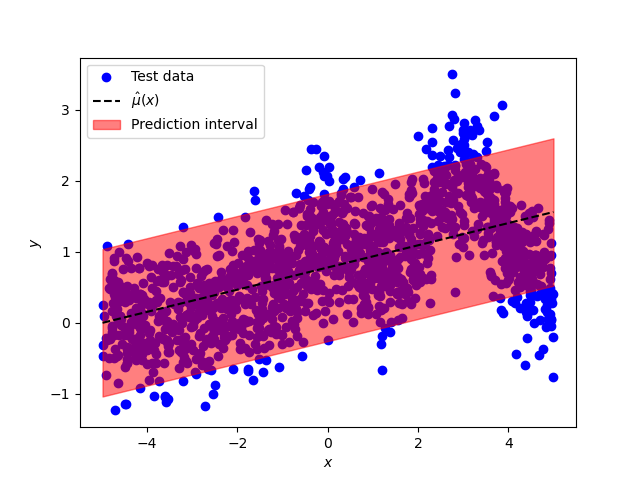
\includegraphics[width=\linewidth]{figures/2_3_LR.png}    
        \caption{Linear regression} \label{fig:2_3_LR}
    \end{subfigure}
    \begin{subfigure}{0.49\textwidth}
        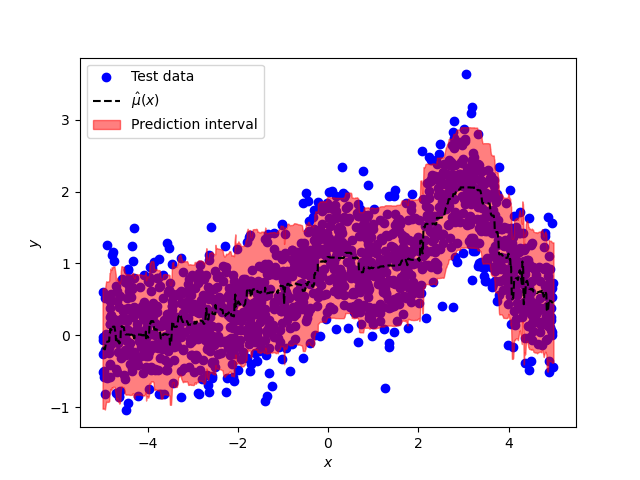
\includegraphics[width=\linewidth]{figures/2_3_RF.png}
        \caption{Random forests} \label{fig:2_3_RF}
    \end{subfigure}
    \begin{subfigure}{0.49\textwidth}
        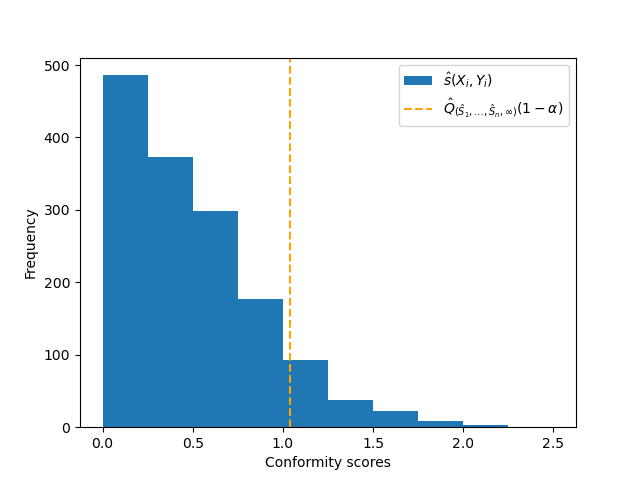
\includegraphics[width=\linewidth]{figures/2_3_LR_scores.png}    
        \caption{Linear regression} \label{fig:2_3_LR_scores}
    \end{subfigure}
    \begin{subfigure}{0.49\textwidth}
        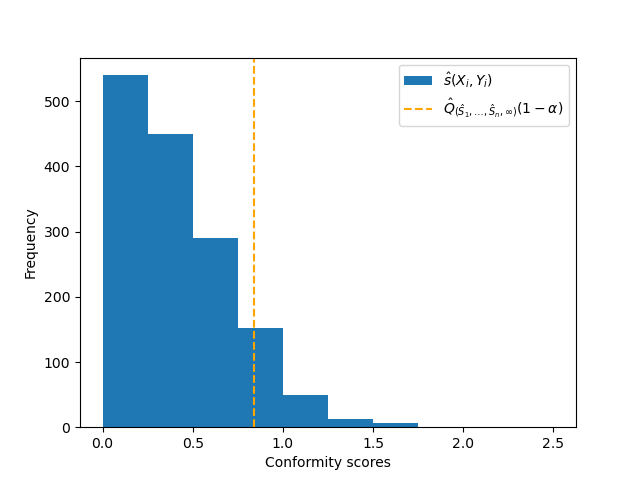
\includegraphics[width=\linewidth]{figures/2_3_RF_scores.png}    
        \caption{Random forests} \label{fig:2_3_RF_scores}
    \end{subfigure}
    \begin{subfigure}{0.49\textwidth}
        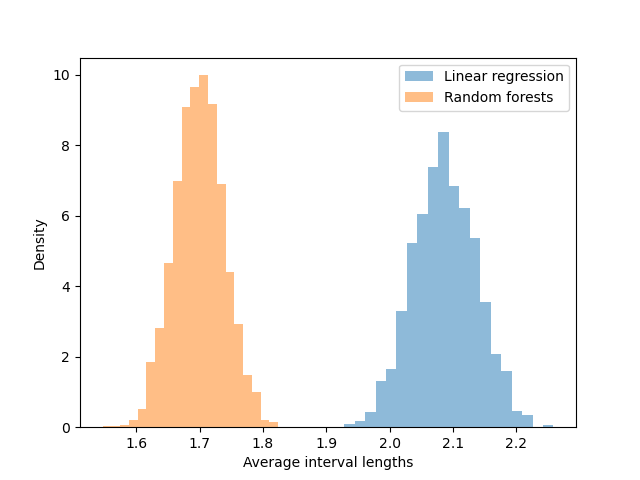
\includegraphics[width=\linewidth]{figures/2_3_lens.png}    
        \caption{Distribution of average prediction interval lengths over \(2000\) independent draws of the calibration and test datasets.} \label{fig:2_3_lens}
    \end{subfigure}
    \caption{First row: plot of split conformal prediction intervals. Second row: histogram of conformity scores. Third row: distribution of average prediction interval length.}
\label{fig:2_3_example}
\end{figure}

% \begin{figure}[H]
%     \centering
%     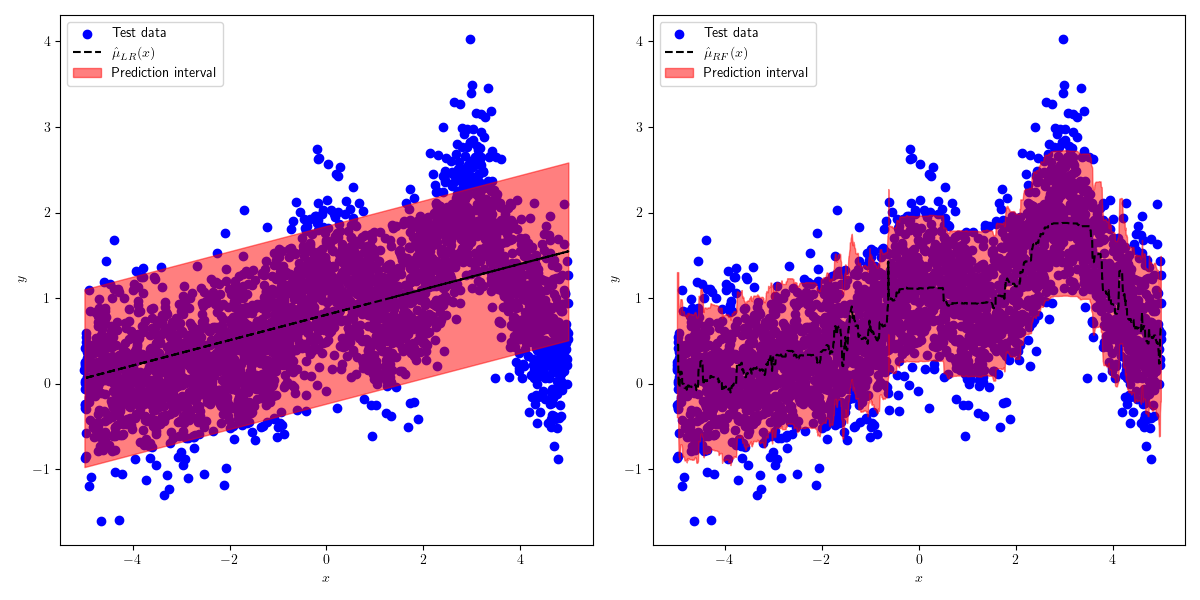
\includegraphics[width=\linewidth]{figures/2_3_LR_RF_example.png}
%     \caption{}
%     \label{fig:split_LR_RF}
% \end{figure}

\subsubsection{Training-conditional coverage}
\label{subsubsec:training_conditional_coverage}

An important observation regarding the coverage guarantee of conformal predicition in both \cref{thm:fullconformal_coverage} and \cref{thm:splitconformal_coverage} is that it provides \textit{marginal coverage}. This refers to the fact that the probability \(\Prob{Y_{n+1} \in C(X_{n+1})}\) is marginalising over \(((X_i, Y_i))_{i=1}^{n+1}.\) One reason why this may be an issue, is that it does not guarantee coverage for any given value of the test predictor \(X_{n+1}\), i.e. it does not guarantee \textit{test-conditional coverage}: \[\Prob{Y_{n+1} \in C(X_{n+1}) \mid X_{n+1}} \geq 1- \alpha.\] This means that conformal prediction could overcover in some regions of \(\mathcal{X}\) and undercover in other regions, whilst still achieving at least \(1-\alpha\) coverage on average. We will see examples of this in \cref{subsec:conformityscore}. Lack of test-conditional coverage is a significant disadvantage of conformal prediction, but we will not discuss it further in this essay. \vskip5pt

\noindent
Instead, we will consider the \textit{training-conditional} coverage \cite{angelopoulos2024theoreticalfoundationsconformalprediction,tibs_advanced_topics} \[\Prob{Y_{n+1} \in C(X_{n+1}) \mid (X_1, Y_1), \ldots, (X_n, Y_n)} \] in this subsection.   Note that this is a random quantity since it is a function of \(((X_i, Y_i))_{i=1}^n\). The presentation of this subsection is inspired by \cite{angelopoulos2021gentle,angelopoulos2024theoreticalfoundationsconformalprediction,tibs_advanced_topics}. \vskip5pt

\noindent
In the case of split conformal prediction, it is possible to exactly derive the distribution of this quantity. We provide our own proof of this result, following the steps outlined in \cite{tibs_advanced_topics_homework}.

\begin{lemma}[\cite{tibs_advanced_topics}]
    Suppose \((X_1, Y_1), \ldots, (X_{n+1}, Y_{n+1})\) are i.i.d. and suppose that (conditional on \(D_\R{tr}\)) \(\hat{S}_i\) has a continuous cumulative distribution function \(F\). Then \[
        \Prob{Y_{n+1} \in C(X_{n+1}) \, | \, D_\R{cal}} \sim \R{Beta}(k_\alpha, n + 1 - k_\alpha), 
    \] where \(k_\alpha = \lceil (1-\alpha)(n+1) \rceil\).
\label{lemma:training_conditional_coverage}
\end{lemma}
\begin{proof}
    Throughout, we work conditional on \(D_\R{tr}\), so that \(\hat{s}\) is fixed. We first claim that if \(U_1, \ldots, U_n \overset{\R{i.i.d.}}{\sim} \R{Uniform}(0,1)\) with order statistics \(U_{(1)} \leq \cdots \leq U_{(n)}, \) then for any \(k \in [n]\), \[U_{(k)} \sim \R{Beta}(k, n+1-k).\] Note that for any \(x \in \mathbb{R}\), we have that \[\Prob{U_{(k)} \leq x} = \sum_{r=k}^{n} \binom{n}{r} x^r (1-x)^{n-r}\] since \(U_{(k)} \leq x\) if and only if at least \(k\) of the random variables \(U_1, \ldots, U_n\) are less than or equal to \(x\). Note also that \(\Prob{U_i \leq x} = x\) for any \(i \in [n]\). Therefore, if \(g(z) = z^r (1-z)^{n-r}\)we have that \begin{align*}
        \lim_{\epsilon \to 0} \frac{\Prob{x \leq U_{(k)} \leq x+\epsilon}}{\epsilon} &= \sum_{r=k}^{n} \lim_{\epsilon \to 0} \, \frac{g(x+\epsilon) - g(x)}{\epsilon} \\
        &= \sum_{r=k}^{n} \binom{n}{r} g'(x) \\
        &= \sum_{r=k}^{n} \binom{n}{r} r x^{r-1}(1-x)^{n-r} - \sum_{r=k}^{n} \binom{n}{r} (n-r) x^{r}(1-x)^{n-r-1} \\
        &= n \sum_{r=k-1}^{n-1} \binom{n-1}{r} r x^{r-1}(1-x)^{n-r} -  n \sum_{r=k}^{n-1} \binom{n-1}{r} (n-r) x^{r}(1-x)^{n-r-1} \\
        &= n \binom{n-1}{k-1} x^{k-1}(1-x)^{n-k},
    \end{align*}
    which is the density of a \(\R{Beta}(k, n+1-k)\) distribution. \vskip5pt

    \noindent
    Let \(F\) be the cumulative distribution function of \(\hat{S}_1, \ldots, \hat{S}_{n+1}.\) It is a standard result (see Appendix, \cref{appendix:results}) that \(F(\hat{S}_1), \ldots, \hat{F}(S_{n+1}) \overset{\R{i.i.d.}}{\sim} \R{Uniform}(0,1).\) Therefore, for any \(k \in [n]\) \begin{align*}
        \Prob{\hat{S}_{n+1} \leq \hat{S}_{(k)} \, | \, D_\R{cal}} = F(\hat{S}_{(k)}) \overset{\R{d}}{=} U_{(k)} \sim \R{Beta}(k, n+1-k)
    \end{align*} since \(F\) is increasing. Finally, we note that \[\Prob{Y_{n+1} \in C(X_{n+1}) \, | \, D_\R{cal}} = \Prob{\hat{S}_{n+1} \leq \hat{S}_{(k_\alpha)} \, | \, D_\R{cal}}, \] and so the result follows.
\end{proof}

\noindent
A further question is as follows: what if we fix the calibration set and compute the empirical coverage on a finite number of test points? \vskip5pt

\noindent
As above, suppose \(D_\R{cal}\) consists of i.i.d. calibration data points, and suppose also that \(\tilde{Z}_1, \ldots, \tilde{Z}_{n_\R{test}} \in \mathcal{Z}\) are i.i.d. test points. Writing \(\tilde{Z}_j = (\tilde{X}_j, \tilde{Y}_j)\), we then have that \begin{align*}
    \frac{1}{n_\R{test}} \sum_{j=1}^{n_\R{test}} \Ind{\tilde{Y}_j \in C(\tilde{X}_j)} \mid D_\R{cal} &\sim \frac{1}{n_\R{test}} \R{Bin}(n_\R{test}, \mu) \\
    \mu &\sim \R{Beta}(k_\alpha, n + 1 - k_\alpha)
\end{align*} by \cref{lemma:training_conditional_coverage}. This means that \[\frac{1}{n_\R{test}} \sum_{j=1}^{n_\R{test}} \Ind{\tilde{Y}_j \in C(\tilde{X}_j)} \sim \frac{1}{n_\R{test}}\R{BetaBin}(n_\R{test}, k_\alpha, n+1-k_\alpha),\] where \(\R{BetaBin}\) is the beta-binomial distribution. We now see that the empirical coverage \eqref{eqn:empirical_cov} is a single draw from this distribution. This result is also discussed in \cite{angelopoulos2021gentle,tibs_advanced_topics}. In the figure below, we plot a histogram of empirical coverages from the numerical example in \cref{subsec:splitconformal} and overlay the beta-binomial probability mass function, illustrating the above result in this example.

\begin{figure}[H]
    \centering
    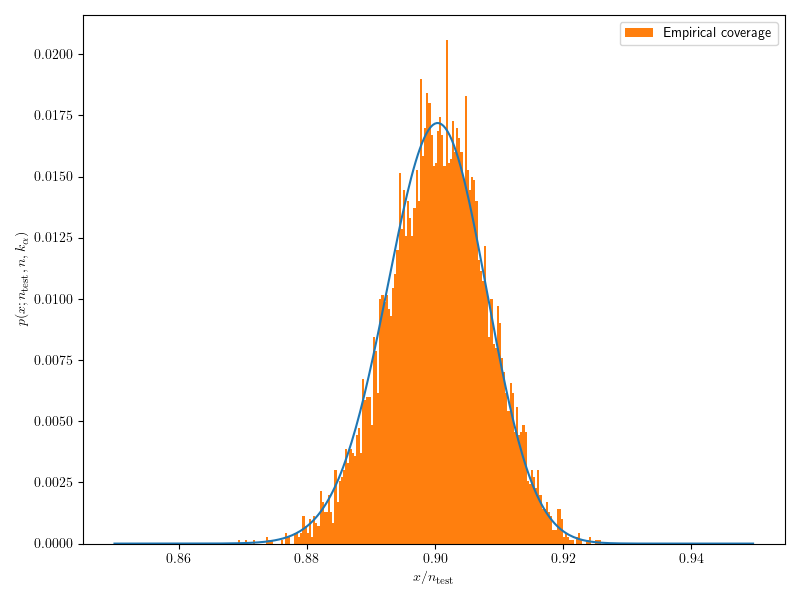
\includegraphics[width=0.6\linewidth]{figures/2_3_training_beta_dist.png}
    \caption{Histogram of \(7000\) samples of the empirical coverage (generated from the example in \cref{subsec:splitconformal}) and the beta-binomial probability mass function overlayed.}
\end{figure}

\subsection{Choice of conformity score}
\label{subsec:conformityscore}

In \cref{subsec:splitconformal}, we showed that any conformity score can be used to construct the split conformal prediction set \eqref{eqn:split_absolute_residual_prediction_set}. However, it is not immediately clear from \eqref{eqn:split_absolute_residual_prediction_set} how the choice of conformity score affects the prediction set. We gain some insight into this from \cref{example:splitCP_absolute_residual_score}, where we see that for split conformal prediction with the absolute residual score, the conformity score influences the width of the prediction interval through the quantile \(\hat{Q}_{(\hat{S}_1, \ldots, \hat{S}_n, \infty)}(1-\alpha)\). In this subsection, we further explore how the choice of conformity score affects the properties of the resulting prediction set. In addition to the absolute residual score, we consider two further examples of conformity scores in the regression setting and compare their empirical performance through numerical experiments. Throughout this subsection, we use split conformal prediction. \vskip5pt

\noindent
We work in the regression setting as in \cref{example:splitCP_absolute_residual_score} with \(\mathcal{X} = \mathbb{R}\). Consider the absolute residual score and its corresponding predicition interval \eqref{eqn:split_absolute_residual_prediction_set}. We observe that a consequence of using the absolute residual score is that the prediction interval has a constant width for all \(x \in \mathbb{R}.\) If the data generating process is heteroscedastic, i.e. \(\R{Var}(Y | X = x)\) is not constant in \(x\), then the prediction interval \eqref{eqn:split_absolute_residual_prediction_set} does not accurately capture the uncertainty in \(Y\) given \(X = x\).The two conformity scores we present aim to make the prediction interval adaptive to heteroscedasticity. 

\subsubsection{Locally Weighted Residual Score}

If \(\hat{\mu}\) is an estimate of the regression function \(\mu:x \mapsto \Exp{Y | X = x}{(}{)}\) and \(\hat{\sigma}\) is an estimate of the \textit{conditional mean absolute deviation} \(x \mapsto \Exp{|Y-\mu(X)| \, \mid X = x}{(}{)}\), then the \textit{locally weighted score} is the conformity score given by \[
    \hat{s}(x,y) = \frac{| y - \hat{\mu}(x)|}{\hat{\sigma}(x)}.
\] The corresponding prediction set is given by \[
    C(x) = \left[ \hat{\mu}(x) - \hat{\sigma}(x) \, \hat{Q}_{(\hat{S}_1, \ldots, \hat{S}_n, \infty)}(1-\alpha), \ \hat{\mu}(x) + \hat{\sigma}(x) \, \hat{Q}_{(\hat{S}_1, \ldots, \hat{S}_n, \infty)}(1-\alpha) \right],
\] using the notation of \cref{subsec:splitconformal}. \vskip5pt

\noindent
This conformity score was originally introduced in \cite{lei2018} and aims to account for heteroscedasticity by scaling the width of the interval in \eqref{eqn:split_absolute_residual_prediction_set} by \(\hat{\sigma}(x)\) for each \(x \in \mathcal{X}\). In practice, \(\hat{\sigma}\) can be estimated by first regressing \(Y_i\) onto \(X_i\) for \((X_i, Y_i) \in D_\R{tr}\) to obtain \(\hat{\mu}\) and then regress \(|Y_i -\hat{\mu}(X_i)|\) onto \(X_i\) for \((X_i, Y_i) \in D_\R{tr}\).

\subsubsection{Conformalised Quantile Regression}

A second approach to generate prediction intervals that are adaptive to heteroscedasticity is to estimate the conditional quantile function \[
    q_{\tau}(x) = \inf \left\{ z \in \mathbb{R}: \Prob{Y \leq z | X = x} \geq \tau \right\}, \quad \tau \in (0,1)
\] directly. This is motivated by noting that \[\Prob{Y \in [q_{\alpha/2}(X), q_{1-\alpha/2}(X)] \ | \  X} = 1-\alpha,\] i.e. the interval \([q_{\alpha/2}(X), q_{1-\alpha/2}(X)]\) has exact \((1-\alpha)-\)level coverage conditional on \(X\). The approach of estimating \(q_\tau(x)\) is referred to as \textit{quantile regression}. In this essay, we do not discuss details of the numerous methods for constructing quantile regression estimators. However, we note the following important fact, which is also discussed in \cite{koenker2005quantile}. \vskip5pt

\noindent
Define the \(\tau-\)\textit{pinball loss} by \(\ell(y, y') = \rho_\tau(y - y')\), where \[\rho_\tau(u) = u(\tau - \Ind{u < 0} ) = \begin{cases}
    u\tau &\quad \text{if } u \geq 0, \\
    u(\tau - 1) &\quad \text{otherwise.}
\end{cases}\]

\begin{lemma}
    Let \(U\) be a real-valued random variable with density \(f\) and strictly increasing cumulative distribution function \(F\). Then for all \(\tau \in (0,1)\), we have that \[F^{-1}(\tau) = \argmin_{t \in \mathbb{R}} \Exp{\ell(Y,t)}{(}{)}\] 
\end{lemma}
\begin{proof}
    We have that \begin{align*}
        \Exp{\ell(Y,t)}{(}{)} = \Exp{\rho_\tau(Y-t)}{(}{)} &= \int_{-\infty}^\infty \rho_\tau(y-t) f(y) \, \R{d}y \\
        &= \int_{-\infty}^t (\tau-1) (y-t) f(y) \, \R{d}y + \int_t^\infty \tau(y-t) f(y) \, \R{d}y.
    \end{align*}
    Equating the derivative of the above expression with respect to \(t\) to \(0\) gives \[\int_{-\infty}^t (1-\tau) f(y) \, \R{d}y - \int_t^\infty \tau f(y) \, \R{d}y = (1-\tau)F(t) - \tau(1-F(t))  =  0,\] which is equivalent to \[t = F^{-1}(\tau).\] The second derivative is equal to \(f(t)\), so \(F^{-1}(\tau)\) is indeed a minimiser.
\end{proof}

\noindent
Therefore, in the same way that training a model with respect to the least-squares loss gives an estimate for the conditional mean, training a model with respect to the \(\tau-\)pinball loss gives an estimate of the \(\tau^{\R{th}}\) quantile of the conditional distribution \(Y|X\). \vskip5pt

\noindent
Using a quantile regression procedure, we may obtain estimates \(\hat{q}_{\alpha/2}(x)\) and \(\hat{q}_{1-\alpha/2}(x)\) for \(q_{\alpha/2}(x)\) and \(q_{1-\alpha/2}(x)\), respectively. However, the interval \([\hat{q}_{\alpha/2}(x), \hat{q}_{1-\alpha/2}(x)]\) is not guaranteed to have \((1-\alpha)-\)level coverage in general. \textit{Conformalised quantile regression} \cite{romano2019_CQR} calibrates this interval using conformal prediction to provide it with a finite-sample coverage guarantee as in \cref{thm:splitconformal_coverage}. \vskip5pt

\noindent
After obtaining estimates \(\hat{q}_{\alpha/2}(x)\) and \(\hat{q}_{1-\alpha/2}(x)\) from the proper training set, conformalised quantile regression applies split conformal prediction with the conformity score \[
    \hat{s}(x,y) = \max\left\{ \hat{q}_{\alpha/2}(x) - y, \, y - \hat{q}_{1-\alpha/2}(x) \right\}.
\] This results in the conformal prediction interval \begin{align*}
    &\left\{ y \in \mathbb{R}: \hat{q}_{\alpha/2}(X_{n+1}) - y \leq \hat{Q}_{(\hat{S}_1, \ldots, \hat{S}_n, \infty)}(1-\alpha) \quad \R{and} \quad y - \hat{q}_{1-\alpha/2}(X_{n+1}) \leq \hat{Q}_{(\hat{S}_1, \ldots, \hat{S}_n, \infty)}(1-\alpha) \right\} \\
    &= \left[\hat{q}_{\alpha/2}(X_{n+1}) - \hat{Q}_{(\hat{S}_1, \ldots, \hat{S}_n, \infty)}(1-\alpha), \hat{q}_{1-\alpha/2}(X_{n+1}) + \hat{Q}_{(\hat{S}_1, \ldots, \hat{S}_n, \infty)}(1-\alpha)  \right].
\end{align*}

\noindent
To intuitively understand this score, we note the following points, inspired by the discussion in \cite{romano2019_CQR}. If \(y < \hat{q}_{\alpha/2}(x)\), i.e. \(y\) is below the predicted lower quantile, then \(\hat{s}(x,y) = |y - \hat{q}_{\alpha/2}(x)|\) is the absolute error compared to the predicted lower quantile. Similarly, if \(y > \hat{q}_{1-\alpha/2}(x)\), then \(\hat{s}(x,y) = |y - \hat{q}_{1-\alpha/2}(x)|.\) In both of these cases, \(\hat{s}(x,y) > 0\), indicating the interval \([\hat{q}_{\alpha/2}(x), \hat{q}_{1-\alpha/2}(x)]\) has failed to cover \(y\), and its value measures the magnitude of the error in the fitted model with respect to \((x,y)\). If \(\hat{q}_{\alpha/2}(x) < y < \hat{q}_{1-\alpha/2}(x)\), i.e. the interval \([\hat{q}_{\alpha/2}(x), \hat{q}_{1-\alpha/2}(x)]\) covers \(y\), then \(\hat{s}(x,y) < 0\) and \[\hat{s}(x,y) = \min \left\{ y - \hat{q}_{\alpha/2}(x), \, \hat{q}_{1-\alpha/2}(x) - y \right\},\] which may be interpreted as the smaller of the two `margins' by which the interval \([\hat{q}_{\alpha/2}(x), \hat{q}_{1-\alpha/2}(x)]\) covers \(y\). We see from the above that if the estimated interval \([\hat{q}_{\alpha/2}(x), \hat{q}_{1-\alpha/2}(x)]\) overcovers, then conformalised quantile regression narrows the interval, and if the estimated interval undercovers, then conformalised quantile regression widens the interval.

\subsubsection{Numerical Experiments}

We now present numerical experiments designed to highlight that the locally weighted score and conformalised quantile regression are more adaptive to heteroscedasticity. We consider two data generating processes. Setting 1 generates i.i.d. data points with homoscedastic noise, and setting 2 generates i.i.d data points with heteroscedastic noise.
\begin{enumerate}[(i)]
    \item \textbf{Setting 1: } \begin{align*}
        X_1, X_2, \ldots &\overset{\R{i.i.d}}{\sim} \R{Uniform}(-5,5) \\
        \epsilon_1, \epsilon_2, \ldots &\overset{\R{i.i.d}}{\sim} \mathcal{N}(0,1) \\
        Y_i &= 1 - X_i + 2\epsilon_i. 
    \end{align*} for all \(i \in [n]\).
    \item \textbf{Setting 2: } \begin{align*}
        X_1, X_2, \ldots &\overset{\R{i.i.d}}{\sim} \R{Uniform}(-5,5) \\
        \epsilon_1, \epsilon_2, \ldots &\overset{\R{i.i.d}}{\sim} \mathcal{N}(0,1) \\
        Y_i &= 1 - X_i + \frac{1}{2}\left(|X_i| + 2\right)\left(\sin(2X_i) + \frac{3}{2}\right) \, \epsilon_i
    \end{align*} for all \(i \in [n]\).    
\end{enumerate}

\noindent
In each setting, we set \(\alpha = 0.1\) and generate i.i.d. proper training, calibration and test datasets with \(1000, 1500, 1500\) datapoints, respectively. We then generate split conformal prediction intervals (using the calibration dataset) for each datapoint in the test dataset and calculate both the empirical coverage (as in \eqref{eqn:empirical_cov}) and the average length of the prediction intervals for the test dataset. We repeat this over \(2000\) independent draws of the calibration and test datasets. We repeat this experiment using the absolute residual score, the locally weighted residual score, conformalised quantile regression and quantile regression. \vskip5pt

\noindent
In \cref{tab:2_4_settings1_2_results}, we record the average empirical coverage and the average length of the prediction intervals, averaged over the \(2000\) draws. 
In \cref{fig:2_4_lens_dists}, we plot a histogram of the average length of the prediction intervals obtained in each of the \(2000\) draws. This estimates the distribution of \[\Exp{|C(X_{n+1}; D_\R{cal})| \mid D_\R{cal}}{[}{]},\] where, in the above display, we make the dependence of the prediction interval on the calibration data \(D_\R{cal}\) explicit, and \(|\cdot|\) denotes the length of the prediction interval. \cref{fig:2_4_homoscedastic} and \cref{fig:2_4_heteroscedastic} plot the prediction intervals obtained using the three different conformity scores, where each plot refers to a single draw of the calibration and test datasets. \vskip5pt

\noindent
From \cref{tab:2_4_settings1_2_results}, we observe that all three conformity scores achieve the target coverage in both settings, as guaranteed by \cref{thm:splitconformal_coverage} since all the data points are i.i.d., and thus exchangeable. However, quantile regression by itself does not give valid coverage. In setting 1, \cref{fig:2_4_lens_dists} shows that three conformity scores give similar distributions for the average length of the prediction intervals. However, in setting 2, we see in \cref{fig:2_4_lens_dists} that the locally weighted score and conformalised quantile regression tend to give much narrower prediction intervals as compared to the absolute residual score. It is clear from \cref{fig:2_4_heteroscedastic} that the width of the prediction intervals \(C(x)\) obtained using the locally weighted residual score and conformalised quantile regression vary with \(x\) to account for the heteroscedasticity. In contrast, the intervals obtained using the absolute residual score have constant width, leading to them overcovering in some regions and undercovering in others.

\begin{table}[H]
    \centering
    \renewcommand{\arraystretch}{1.2}
    \begin{tabular}{|p{1.2cm}|p{1.5cm}|p{1.5cm}|p{1.5cm}|p{1.5cm}|p{1.5cm}|p{1.5cm}|p{1.5cm}|p{1.5cm}|}
        \hline
        & \multicolumn{2}{c|}{Absolute residual} & \multicolumn{2}{c|}{Locally weighted} & \multicolumn{2}{p{3.5cm}|}{Conformalised quantile regression} & \multicolumn{2}{c|}{Quantile regression} \\
        \hline
        & Average coverage & Average length & Average coverage & Average length & Average coverage & Average length & Average coverage & Average length\\
        \hline
        Setting 1 & 0.90022 & 6.6991 & 0.90008 & 6.7815 & 0.90028 & 6.8889 & 0.86825 & 6.3046 \\
        \hline
        Setting 2 & 0.90024 & 13.146 & 0.90012 & 11.305 & 0.90015 & 11.595 & 0.87957 & 10.814 \\
        \hline
    \end{tabular}
    \caption{Average coverage and average length of the conformal prediction intervals on the test dataset}
    \label{tab:2_4_settings1_2_results}
\end{table}

\begin{figure}[H]
    \centering
    \begin{subfigure}{0.49\textwidth}
    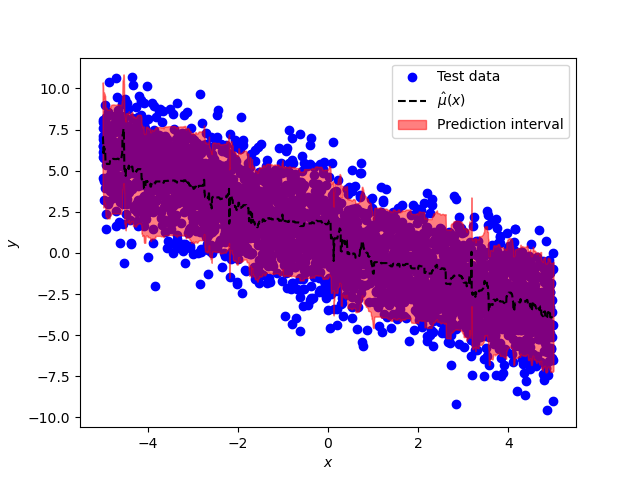
\includegraphics[width=\linewidth]{figures/2_4_homoscedastic_RF.png}    
    \caption{Absolute residual score} \label{fig:2_4_homoscedastic_RF}
    \end{subfigure}
    \begin{subfigure}{0.49\textwidth}
    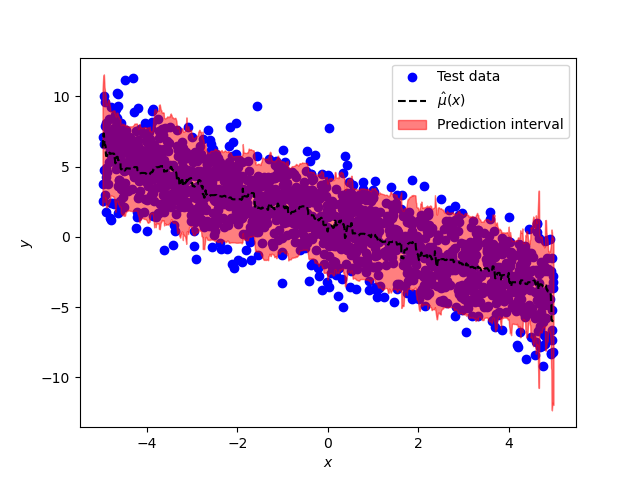
\includegraphics[width=\linewidth]{figures/2_4_homoscedastic_LW.png}
    \caption{Locally weighted score} \label{fig:2_4_homoscedastic_LW}
    \end{subfigure}
    \begin{subfigure}{0.49\textwidth}
    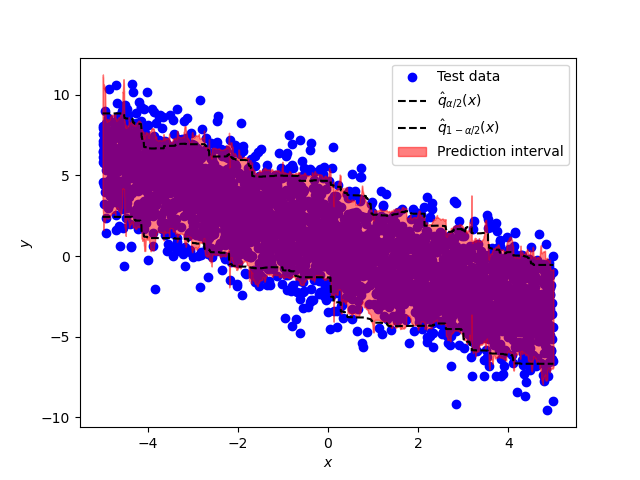
\includegraphics[width=\linewidth]{figures/2_4_homoscedastic_CQR.png}    
    \caption{Conformalised quantile regression} \label{fig:2_4_homoscedastic_CQR}
    \end{subfigure}
    \caption{Conformal prediction intervals in setting 1.}
\label{fig:2_4_homoscedastic}
\end{figure}

\begin{figure}[H]
    \centering
    \begin{subfigure}{0.49\textwidth}
    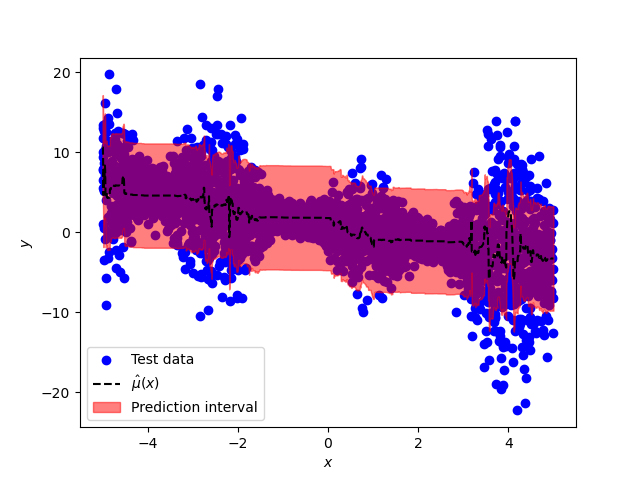
\includegraphics[width=\linewidth]{figures/2_4_heteroscedastic_RF.png}    
    \caption{Absolute residual score} \label{fig:2_4_heteroscedastic_RF}
    \end{subfigure}
    \begin{subfigure}{0.49\textwidth}
    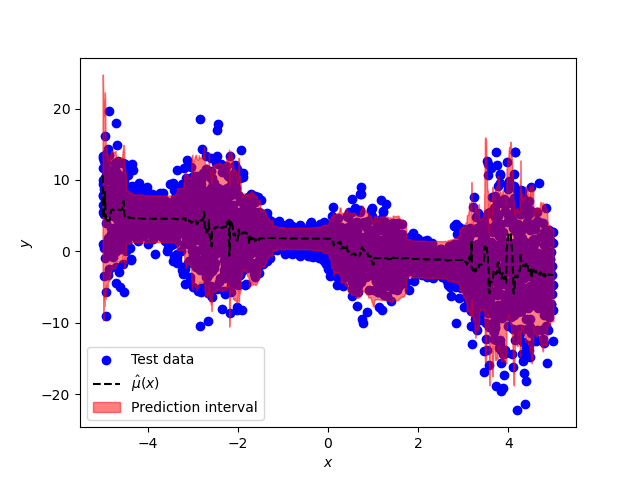
\includegraphics[width=\linewidth]{figures/2_4_heteroscedastic_LW.png}
    \caption{Locally weighted score} \label{fig:2_4_heteroscedastic_LW}
    \end{subfigure}
    \begin{subfigure}{0.49\textwidth}
    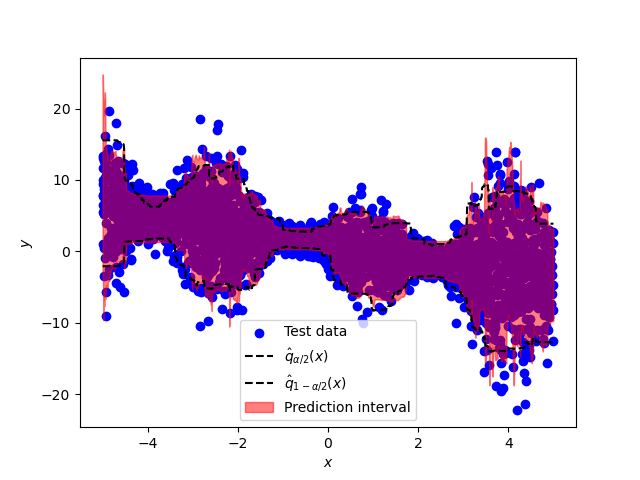
\includegraphics[width=\linewidth]{figures/2_4_heteroscedastic_CQR.png}    
    \caption{Conformalised quantile regression} \label{fig:2_4_heteroscedastic_CQR}
    \end{subfigure}
    \medskip
    \caption{Conformal prediction intervals in setting 2.}
\label{fig:2_4_heteroscedastic}
\end{figure}

\begin{figure}[H]
    \vspace{-0.8cm}
    \centering
    \begin{subfigure}{0.47\textwidth}
        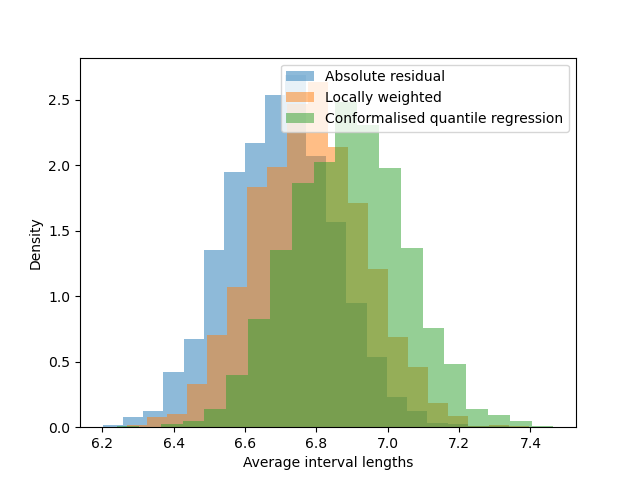
\includegraphics[width=\linewidth]{figures/2_4_lens_dist.png}    
        \caption{Setting 1} \label{fig:2_4_homoscedastic_lens_dist}
    \end{subfigure}
    \begin{subfigure}{0.47\textwidth}
        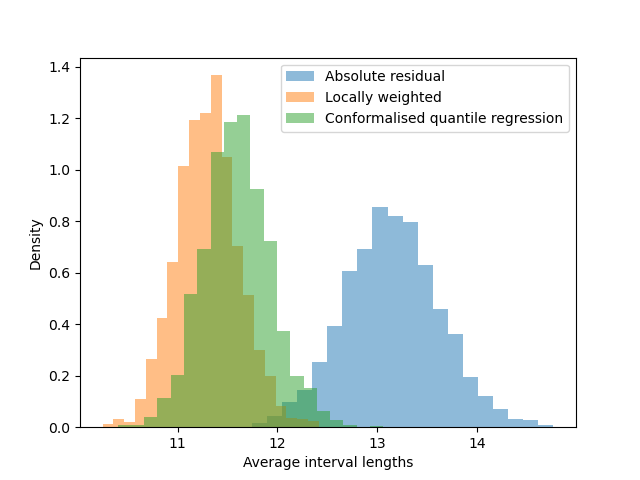
\includegraphics[width=\linewidth]{figures/2_4_heteroscedastic_lens_dist.png}    
        \caption{Setting 2} \label{fig:2_4_heteroscedastic_lens_dist}
    \end{subfigure}
    \caption{Distribution of average prediction interval lengths from \(2000\) independent draws of calibration and test datasets.}
\label{fig:2_4_lens_dists}
\end{figure}


\section{Extensions of Conformal Prediction}
\label{sec:extensions_of_CP}

In this section, we explore three theoretical extensions to the conformal prediction framework presented in \cref{sec:foundations_of_CP}. As the proof of \cref{thm:fullconformal_coverage} demonstrates, exchangeability is a fundamental assumption for the validity of conformal prediction. In many real-world applications, exchangeability may not hold. A key example of this is distribution shift, a setting where the test data has a different distribution to the training data. In \cref{subsec:nex_CP}, we consider the case where exchangeability does not hold and present a conformal prediction procedure developed by \cite{barber2023conformalbeyondexch} that provides a coverage guarantee in this setting. The specific case of distribution shift is subsequently analysed in \cref{subsec:dist_shift}. To conclude this section, we return to the setting of exchangeability but consider an extension of conformal prediction, developed by \cite{angelopoulos2024riskcontrol}, that imparts a more general class of guarantees to conformal prediction sets.

\subsection{Nonexchangeable Conformal Prediction}
\label{subsec:nex_CP}



In this subsection, we present the \textit{nonexchangeable conformal prediction} (NexCP) method developed in \cite{barber2023conformalbeyondexch}. Full conformal prediction relies on two main assumptions: the exchangeability of the data and the symmetry of the conformity score. The key contribution of \cite{barber2023conformalbeyondexch}, presented in \cref{thm:nexCP_coverage}, is deriving a modification of the full conformal prediction procedure that has a coverage guarantee when both of these assumptions are violated. \vskip5pt

\noindent
The key theoretical insight to extend conformal prediction beyond exchangeability, that is common to both the NexCP method and the method presented in \cref{subsec:dist_shift}, is to introduce weights. We will compare the NexCP method and the method in \cref{subsec:dist_shift} at the end of \cref{subsec:dist_shift}.  Recall that we introduced the notion of weighted quantiles \(\hat{Q}_z^w(1-\alpha)\) in \cref{defn:empirical_cdfquantile} but specialised to the case where the weights are all equal in the results of \cref{sec:foundations_of_CP}. The NexCP method assigns fixed weights \(w_1, \ldots, w_{n} \in [0, \infty)\) to the data points \((X_1, Y_1), \ldots, (X_n, Y_n)\), respectively. The corresponding normalised weights are defined by \begin{equation}
    \tilde{w_i} = \frac{w_i}{1+\sum_{j=1}^n w_j} \quad \mathrm{and} \quad \tilde{w}_{n+1} = \frac{1}{1+\sum_{j=1}^n w_j}
\label{eqn:nexCP_weights_defn}
\end{equation} for all \(i \in [n]\). \vskip5pt

\noindent
Before we present the main theorem of this subsection, we introduce the required notation. Given data points \((X_1, Y_1), \ldots, (X_{n+1}, Y_{n+1}) \in \mathcal{Z}\), \(y \in \mathcal{Y}\) and \(k \in [n+1]\), we define \[D = ((X_i, Y_i))_{i=1}^{n+1}, \quad D^{y} = ((X_i, Y_i)_{i=1}^n, (X_{n+1}, y)), \quad \quad D^{(k)} = \pi_k(D), \quad \mathrm{and} \quad D^{y, (k)} = \pi_k(D^{y}). \] where \(\pi_k \in S_{n+1}\) is the transposition exchanging \(k\) and \(n+1\). \vskip5pt

\noindent
Let \(s\) be a conformity score. As mentioned above, we will not assume that \(s\) is symmetric. Therefore, the model fitting procedure within the conformity score may take the order of the data points into account. We define \[S = (s((X_i, Y_i); D))_{i=1}^{n+1}, \quad \mathrm{and} \quad S^{(k)} = ( s(( X_{\pi_k(i)}, Y_{\pi_k(i)} ); D^{(k)}) )_{i=1}^{n+1}.\] We also define \[S_i^{y, (k)} = \begin{cases}
    s(( X_i, Y_i ); D^{y, (k)}) \quad &\mathrm{if} \ i = 1, \ldots, n \\
    s(( X_{n+1}, y ); D^{y, (k)}) \quad &\mathrm{if} \ i = n+1,
\end{cases} \quad \mathrm{and} \quad S^{y, (k)} = (S_i^{y,(k)})_{i=1}^{n+1}.\]

\noindent
We define \(K\) to be random variable taking values in \([n+1]\) such that \begin{equation}
    \Prob{K = k} = \tilde{w}_k
\label{eqn:nexCP_K_defn}
\end{equation} for all \(k \in [n+1]\), and we take \(K\) and \(D\) to be independent. \vskip5pt

\noindent
We also recall the definition of the total variation distance.

\begin{definition}
    Let \(U\) and \(V\) be random variables. The \textit{total variation distance} between \(U\) and \(V\) is defined as \[\R{d_{TV}}(U,V) = \sup_{A} | \Prob{U \in A} - \Prob{V \in A}|, \] where the supremum is taken over all measurable sets \(A\). 
\label{defn:TV_distance}
\end{definition}

\noindent
We now prove the main theorem of this subsection which provides the predicition set and coverage guarantee for the NexCP method.

\begin{theorem}
    Let \((X_1, Y_1), \ldots, (X_{n+1}, Y_{n+1}) \in \mathcal{Z}\) be a sequence of data points and \(s\) be a conformity score. Let \(w_1, \ldots, w_{n+1} \in [0, \infty)\) be fixed real numbers and define \(\tilde{w}_i\) according to \eqref{eqn:nexCP_weights_defn} for all \(i \in [n+1]\). Let \(K\) be a random variable as in \eqref{eqn:nexCP_K_defn} that is independent of \(D\). Define the prediction set \[
        C(X_{n+1}) = \left\{ y \in \mathcal{Y} : \ S_{n+1}^{y, (K)} \leq \hat{Q}_{S^{y, (K)}}^{\tilde{w}}(1-\alpha)  \right\}.
    \] Then we have that \begin{equation}
        \Prob{Y_{n+1} \in C(X_{n+1})}  \geq 1-\alpha - \sum_{k=1}^n \tilde{w}_k \R{d_{TV}}(S, S^{(k)}).
    \end{equation}
\label{thm:nexCP_coverage}
\end{theorem}
\begin{proof}
    If \(Y_{n+1} \not \in C(X_{n+1})\), then \[S_{n+1}^{Y_{n+1}, (K)} > \hat{Q}^{\tilde{w}}_{S_{n+1}^{Y_{n+1}, (K)}}(1-\alpha).\] This implies that \[S_{n+1}^{Y_{n+1}, (K)} > \hat{Q}^{\tilde{w}}_{\left( S_1^{Y_{n+1}, (K)}, \ldots, S_n^{Y_{n+1}, (K)}, \infty  \right)}(1-\alpha)\] by \cref{lemma:quantile_lemma}. We now claim that \[\hat{Q}^{\tilde{w}}_{\left( S_1^{Y_{n+1}, (K)}, \ldots, S_n^{Y_{n+1}, (K)}, \infty  \right)}(1-\alpha) \geq \hat{Q}^{\tilde{w}}_{S^{(K)}}(1-\alpha).\] If \(K = n+1\), then this follows by \eqref{eqn:quantile_lemma_pt1} in the proof of \cref{lemma:quantile_lemma}. If \(K \leq n\), we have that for any \(x \in \mathbb{R}\), \begin{align*}
        \hat{F}^{\tilde{w}}_{S^{(K)}}(x) &= \sum_{i=1}^{n+1} \tilde{w}_i \Ind{x \geq S_{\pi_K(i)}^{Y_{n+1}, (K)}} \\
        &= \sum_{\substack{i = 1 \\ i \neq K}}^{n} \tilde{w}_i \Ind{x \geq S_i^{Y_{n+1}, (K)}} + \tilde{w}_K \Ind{x \geq S_{n+1}^{Y_{n+1}, (K)}} + \tilde{w}_{n+1} \Ind{x \geq S_K^{Y_{n+1}, (K)}} \\
        &= \hat{F}^{\tilde{w}}_{\left( S_1^{Y_{n+1}, (K)}, \ldots, S_n^{Y_{n+1}, (K)}, \infty  \right)}(x) + \tilde{w}_K \Ind{x \geq S_{n+1}^{Y_{n+1}, (K)}} + \tilde{w}_{n+1} \Ind{x \geq S_K^{Y_{n+1}, (K)}} \\
        & \hspace{4.8cm} -  \tilde{w}_K \Ind{x \geq S_{K}^{Y_{n+1}, (K)}} - \tilde{w}_{n+1} \Ind{x \geq \infty} \\
        &= \hat{F}^{\tilde{w}}_{\left( S_1^{Y_{n+1}, (K)}, \ldots, S_n^{Y_{n+1}, (K)}, \infty  \right)}(x) + \tilde{w}_K \left( \Ind{x \geq S_{n+1}^{Y_{n+1}, (K)}} - \Ind{x \geq \infty} \right) \\
        & \hspace{4.8cm} + \left( \tilde{w}_{n+1} - \tilde{w}_K\right) \left(\Ind{x \geq S_{K}^{Y_{n+1}, (K)}} - \Ind{x \geq \infty} \right) \\
        & \geq \hat{F}^{\tilde{w}}_{\left( S_1^{Y_{n+1}, (K)}, \ldots, S_n^{Y_{n+1}, (K)}, \infty  \right)}(x).
    \end{align*}
    Therefore, we have that \[\hat{F}^{\tilde{w}}_{S^{(K)}}\left( \hat{Q}^{\tilde{w}}_{\left( S_1^{Y_{n+1}, (K)}, \ldots, S_n^{Y_{n+1}, (K)}, \infty  \right)}(1-\alpha) \right) \geq 1-\alpha,\] by \cref{lemma:cdfquantile} which shows the claim above. \vskip5pt

    \noindent
    So far, we have shown that \[Y_{n+1} \not \in C(X_{n+1}) \implies S_{n+1}^{Y_{n+1}, (K)} >\hat{Q}^{\tilde{w}}_{S^{(K)}}(1-\alpha).\] Noting that \(S_{n+1}^{Y_{n+1}, (K)} = S_K^{(K)}\), this implies that \[\Prob{Y_{n+1} \in C(X_{n+1}) } \geq \Prob{ S_K^{(K)} \leq \hat{Q}^{\tilde{w}}_{S^{(K)}}(1-\alpha) }. \]
    \noindent
    Thus, we have that
    \begin{align*}
        \Prob{Y_{n+1} \in C(X_{n+1})} &\geq \Prob{ S_K^{(K)} \leq \hat{Q}^{\tilde{w}}_{S^{(K)}}(1-\alpha) } \\
        &= \sum_{k=1}^{n+1} \Prob{S_k^{(k)} \leq \hat{Q}^{\tilde{w}}_{S^{(k)}}(1-\alpha), \, K=k} \\
        &= \sum_{k=1}^{n+1} \tilde{w}_k \Prob{S_k^{(k)} \leq \hat{Q}^{\tilde{w}}_{S^{(k)}}(1-\alpha)} \\
        &= \sum_{k=1}^{n+1} \tilde{w}_k \Prob{S_k \leq \hat{Q}^{\tilde{w}}_{S}(1-\alpha)} \\
        & \hspace{2.6cm} + \sum_{k=1}^{n+1} \tilde{w}_k \left[ \Prob{S_k^{(k)} \leq \hat{Q}^{\tilde{w}}_{S^{(k)}}(1-\alpha)} - \Prob{S_k \leq \hat{Q}^{\tilde{w}}_{S}(1-\alpha)} \right] \\
        &\geq \Exp{\sum_{k=1}^{n+1} \tilde{w}_k \Ind{S_k \leq \hat{Q}^{\tilde{w}}_{S}(1-\alpha)}}{[}{]} - \sum_{k=1}^{n+1} \tilde{w}_k \, \R{d_{TV}}(S, S^{(k)}) \\
        &= \Exp{\hat{F}^{\tilde{w}}_S(\hat{Q}^{\tilde{w}}_S (1-\alpha))}{[}{]} - \sum_{k=1}^{n+1} \tilde{w}_k \, \R{d_{TV}}(S, S^{(k)}) \\
        &\geq 1-\alpha - \sum_{k=1}^{n+1} \tilde{w}_k \, \R{d_{TV}}(S, S^{(k)}),
    \end{align*}
    where the third line follows from the independence of \(K\) and \(D\), the fifth line follows from \cref{defn:TV_distance} and the final inequality follows from \cref{lemma:cdfquantile}.
\end{proof}

\noindent
The corresponding algorithm, referred to as \textit{nonexchangeable full conformal predicition} is stated below.

\begin{algorithm}[H]
    \label{alg:nexCP}
    \caption{Nonexchangeable full conformal prediction algorithm}
    \begin{algorithmic}
        \Require Calibration \(((X_i, Y_i))_{i=1}^n\); test predictor \(X_{n+1}\); miscoverage level \(\alpha \in (0,1)\), conformity score \(\hat{s}\). 
        \State Initialise \(C \gets \emptyset\)
        \State Draw \(K\) from \([n+1]\) according to \eqref{eqn:nexCP_K_defn}.

        \For{\(y \in \mathcal{Y}\)}
            \State Compute \(S_i^{y, (K)}\) for \(i \in [n+1]\)
            \State Compute \(\hat{Q}^{\tilde{w}}_{S^{y, (K)}}(1-\alpha)\)
            \If{\(S_{n+1}^{y, (K)} \leq \hat{Q}^{\tilde{w}}_{S^{y, (K)}}\)}
                \State \(C \gets C \cup \{y\}\)
            \EndIf
        \EndFor
        \Ensure \(C\)
    \end{algorithmic}
\end{algorithm}

\noindent
In the same way that split conformal prediction is shown to be a special case of full conformal prediction in \cref{sec:foundations_of_CP}, we may derive a corresponding result for NexCP, referred to as \textit{nonexchangeable split conformal predicition}. We use the notation from \cref{subsec:splitconformal}, denoting \(\hat{s}:\mathcal{X} \to \mathcal{Y}\) to be the conformity score and \(D_\R{tr}\) the proper training set. We also write \(\hat{S}_i = \hat{s}(X_i, Y_i)\) for all \(i \in [n]\) and \(\hat{S}_{n+1}^y = \hat{s}(X_{n+1}, y)\).

\begin{corollary}
    Suppose \((X_1, Y_1), \ldots, (X_n, Y_n), (X_{n+1}, Y_{n+1}) \in \mathcal{Z}\) are data points. Define the prediction set \[
        C(X_{n+1}) = \left\{ y \in \mathcal{Y}: \  \hat{S}_{n+1}^y \leq \hat{Q}^{\tilde{w}}_{(\hat{S}_1, \ldots, \hat{S}_n, \infty)}(1-\alpha)  \right\}.
    \] Then we have that \[\Prob{Y_{n+1} \in C(X_{n+1})}  \geq 1-\alpha - \sum_{k=1}^n \tilde{w}_k \R{d_{TV}}(S, S^{(k)}).\]
\label{corr:nexCP_split}
\end{corollary}
\begin{proof}
    This follows from \cref{thm:nexCP_coverage} and \cref{lemma:quantile_lemma} in exactly the same way as in the proof of \cref{thm:splitconformal_coverage} by taking \(s((x,y); \tilde{D}) = \hat{s}(x,y)\) for \((x,y) \in \mathcal{Z}\) and \(\tilde{D} = \cup_{j \geq 1} \mathcal{Z}^j.\)
\end{proof}

\noindent
We now discuss the implications of \cref{thm:nexCP_coverage}. As mentioned at the beginning of this subsection, the coverage guarantee in \cref{thm:nexCP_coverage} makes no assumption on the distribution of the data or on the conformity score. The quantity \[
    \sum_{k=1}^{n} \tilde{w}_k \R{d_{TV}}(S, S^{(k)}).
\] may be interpreted as the loss in coverage that occurs due to not assuming exchangeability or that the conformity score is symmetric. As in \cite{barber2023conformalbeyondexch}, we can further understand the result by highlighting some important special cases. We record these are corollaries below.

\begin{corollary}
    Let \((X_1, Y_1), \ldots, (X_{n+1}, Y_{n+1}) \in \mathcal{Z}\) and \(s\) be a symmetric conformity score. Let \(C(X_{n+1})\) be the prediction set \eqref{eqn:fullconformal_prediction_set}. Then we have that \[
        \Prob{Y_{n+1} \in C(X_{n+1})}  \geq 1-\alpha - \frac{1}{n+1} \sum_{k=1}^{n} \R{d_{TV}}(S, S^{(k)}).
    \]
\label{corr:nexCP_robustness}
\end{corollary}
\begin{proof}
    Since \(s\) is symmetric, we have that \(S_{i}^{y, (K)} = s((X_i, Y_i); D^{y, (K)}) = s((X_i, Y_i); D^{y}) = S_i^y\) for \(i \in [n]\) and similarly, \(S_{n+1}^{y, (K)} = S_{n+1}^y\). Moreover, if we take \(w_i = 1\) for each \(i \in [n]\), then the prediction set \eqref{eqn:nexCP_prediction_set} coincides with \eqref{eqn:fullconformal_prediction_set}, so the result follows from \cref{thm:nexCP_coverage}.
\end{proof}

\begin{corollary}
    Let \((X_1, Y_1), \ldots, (X_{n+1}, Y_{n+1}) \in \mathcal{Z}\) be exchangeable and \(s\) be a conformity score. With \(\tilde{w}\) and \(K\) as in \cref{thm:nexCP_coverage}, define the prediction set \[C(X_{n+1}) = \left\{ y \in \mathcal{Y} : \ S_{n+1}^{y, (K)} \leq \hat{Q}_{S^{y, (K)}}^{\tilde{w}}(1-\alpha)  \right\}.\] Then we have that \[
        \Prob{Y_{n+1} \in C(X_{n+1})}  \geq 1-\alpha.
    \]
\label{corr:nexCP_exchangeable}
\end{corollary}
\begin{proof}
    If the data is exchangeable, then \(S \overset{d}{=} S^{(k)}\) for any \(k \in [n] \), so \[\sum_{k=1}^n \tilde{w_k} \R{d_{TV}}(S, S^{(k)}) = 0,\] and the result follows from \cref{thm:nexCP_coverage}.
\end{proof}

\noindent
An interpretation of \cref{corr:nexCP_robustness} is that if we apply the standard full conformal prediction algorithm \cref{alg:fullconformal} to nonexchangeable data, then \[\frac{1}{n+1} \sum_{k=1}^{n} \R{d_{TV}}(S, S^{(k)})\] is the loss in marginal coverage compared to the \(1-\alpha\) level in the exchangeable case. If we interpret the quantity in the above display as quantifying the extent to which exchangeability is violated, then \cref{corr:nexCP_robustness} shows that if the violation of exchangeability is small, then the coverage loss from applying standard conformal prediction is small too. \vskip5pt

\noindent
As mentioned in \cite{barber2023conformalbeyondexch}, \cref{corr:nexCP_exchangeable} demonstrates that using the NexCP method does not lead to a loss of coverage in the case that the data is exchangeable. In fact, taking \(w_i = 1\) for each \(i \in [n]\), \cref{corr:nexCP_exchangeable} shows precisely how the full conformal prediction set must be modified in order that the coverage guarantee holds for conformity scores that are not necessarily symmetric. We note that extending full conformal prediction to include non-symmetric conformity scores is useful theoretically since it enables fitting algorithms that do not treat the data symmetrically (e.g. weighted regression) in full conformal prediction. However, since full conformal prediction is rarely used in practice, and split conformal prediction is valid with any conformity score function, the extension to nonsymmetric scores may have limited practical applicability. \vskip5pt

\noindent
Overall, the primary strengths of the NexCP method is that it quantifies the loss of coverage when exchangeability and the symmetry of the score function fail to hold and that it provides extensions of the results in \cref{sec:foundations_of_CP} in the exchangeable case. The main limitation of this method is that it provides no way of choosing the weights. From \cref{thm:nexCP_coverage}, we see that the result is only meaningful if the weights can be suitably chosen to ensure the loss of coverage is small. Whilst the authors of \cite{barber2023conformalbeyondexch} leave the problem of choosing the weights open, they show the following result (\cite{barber2023conformalbeyondexch} Lemma 1). If \(Z_1, \ldots, Z_{n+1}\) are independent, then \[\sum_{k=1}^{n} \tilde{w}_k \R{d_{TV}}(S, S^{(k)}) \leq 2 \sum_{k=1}^{n} \tilde{w}_k \R{d_{TV}}(Z_i, Z_{n+1}).\] This supports the intuition that assigning a higher weight to points whose distribution is similar to the test point yields a smaller loss in coverage.

\subsection{Distribution Shift}
\label{subsec:dist_shift}

Having considered a general violation of exchangeability in \cref{subsec:nex_CP}, in this subsection, we focus on distribution shift. Specifically, denoting \(Z_i = (X_i, Y_i) \in \mathcal{Z}\) for \(i \in [n+1]\), we will consider the case where the calibration data satisfies \(Z_1, \ldots, Z_n \overset{\R{i.i.d.}}{\sim} P\) for a distribution \(P\) and the test point \(Z_{n+1} \sim Q\) for some other distribution \(Q\). Note that \(Z_1, \ldots, Z_{n+1}\) are not exchangeable since they are not identically distributed. The main theorem of this subsection, \cref{thm:dist_shift_coverage}, demonstrates that a modified conformal prediction procedure achieves \((1-\alpha)-\)level coverage in this setting. We will refer to this procedure as \textit{weighted conformal prediction}. \vskip5pt

\noindent
The main ideas for the procedure we discuss were developed in \cite{tibshirani2019covariateshift, ramdas2021labelshift}. Our presentation - inspired by \cite{angelopoulos2024theoreticalfoundationsconformalprediction} - will incorporate some ideas from the more recent works \cite{barber2024finetti,tang2023finiteweighted}, which develops theory to frame the concepts of \cite{tibshirani2019covariateshift,ramdas2021labelshift} more generally. \vskip5pt

\noindent
We first introduce a notion that generalises exchangeability, referred to as \textit{weighted exchangeability} \cite{tibshirani2019covariateshift,barber2024finetti,tang2023finiteweighted}. In the following, \(\mathcal{U}\) denotes a separable complete metric space, \(\mathcal{B}(\mathcal{U})\) denotes the Borel \(\sigma-\)algebra on \(\mathcal{U}\) and \(\Lambda\) denotes the set of measurable functions from \(\mathcal{U}\) to \((0, \infty)\).  The conditions on \(\mathcal{U}\) are required due to measure-theoretic results ensuring the existence of regular conditional distributions, which we do not discuss further here (see Appendix A.1 \cite{barber2024finetti}). 

\begin{definition}[\cite{barber2024finetti,tang2023finiteweighted}]
    \begin{enumerate}[(i)] \itemsep0em
        \item A probability measure \(Q\) on \(\mathcal{U}^n\) is \textit{exchangeable} if for all \(A_1, \ldots, A_n \in \mathcal{B}(\mathcal{U})\), \[Q(A_1 \times \cdots \times A_n) = Q(A_{\sigma(1)} \times \cdots \times A_{\sigma(n)})\] for all \(\sigma \in S_n.\) 
        \item Given \(\lambda = (\lambda_1, \ldots, \lambda_n) \in \Lambda^n\), a probability measure \(Q\) on \(\mathcal{U}^n\) is called \(\lambda-\)\textit{weighted exchangeable} if the measure \(\bar{Q}\) defined as \[\bar{Q}(B) = \int_{B} \frac{\R{d}Q(x_1, \ldots, x_n)}{\lambda_1(x_1) \cdots \lambda_n(x_n)}, \quad \mathrm{for} \ B \in \mathcal{B}(\mathcal{U}^n), \] is exchangeable.
    \end{enumerate}
\label{defn:weighted_exch}
\end{definition}

\noindent
This relates our standard notion of exchangeability by noting that \(U_1, \ldots, U_n\) are exchangeable according to \cref{defn:exch} if and only if \(\mathbb{P} \circ U^{-1}\) is exchangeable according to \cref{defn:weighted_exch}, where \(U = (U_1, \ldots, U_n)\). Moreover, note that \(Q\) is exchangeable if and only if \(Q\) is \(\lambda-\)weighted exchangeable for \(\lambda_1, \ldots, \lambda_n \equiv 1\). We also note that the notion of weighted exchangeability above generalises the definition in \cite{tibshirani2019covariateshift}, which we record below.

\begin{definition}[\cite{tibshirani2019covariateshift}]
    Suppose \(U_1, \ldots, U_n\) are continuous real-valued random variables with joint density \(f\). They are said to be \(\lambda-\)\textit{weighted-exchangeable} if \[f(u_1, \ldots, u_n) = g(u_1, \ldots, u_n) \, \prod_{i=1}^n \lambda(u_i),\] for some \(g\) satisfying \(g(u_1, \ldots, u_n) = g(u_{\sigma(1)}, \ldots, u_{\sigma(n)})\) for all \(u_1, \ldots, u_n \in \mathbb{R}\) and \(\sigma \in S_{n}\).
\label{defn:tibs_weighted_exch}
\end{definition}

\noindent
Specifically, \( U_1, \ldots, U_n\) are \(\lambda-\)weighted-exchangeable according to \cref{defn:tibs_weighted_exch} if and only if \(\mathbb{P} \circ U^{-1}\) is \(\lambda-\)weighted-exchangeable according to \cref{defn:weighted_exch}, where \(U = (U_1, \ldots, U_n)\). Indeed, defining \(g(u_1, \ldots, u_n) = \frac{f(u_1, \ldots, u_n)}{\lambda_1(u_1) \cdots \lambda_n(u_n)}\), we note that for any Borel-measurable \(B_1, \ldots, B_n \subseteq \mathbb{R}\) and \(\sigma \in S_n\), we have \begin{align*}
    \int_{B_1 \times \cdots \times B_n}\frac{\R{d}(\mathbb{P} \circ U^{-1})(u_1, \ldots, u_n)}{\lambda_1(u_1) \cdots \lambda_n(u_n)} = \int_{B_1 \times \cdots \times B_n} g(u_1, \ldots, u_n) \, \R{d}u_1 \cdots \R{d}u_n,
\end{align*}
\noindent
and
\begin{align*}
    &\int_{B_{\sigma(1)} \times \cdots \times B_{\sigma(n)}}\frac{\R{d}(\mathbb{P} \circ U^{-1})(u_1, \ldots, u_n)}{\lambda_1(u_1) \cdots \lambda_n(u_n)} \\
    &= \int_{\mathbb{R}^n} g(u_1, \ldots, u_n) \, \Ind{(u_{\sigma^{-1}(1)}, \ldots, u_{\sigma^{-1}(n)}) \in B_1 \times \cdots \times B_n} \, \R{d}u_{\sigma^{-1}(1)} \cdots \R{d}u_{\sigma^{-1}(n)} \\
    &= \int_{B_1 \times \cdots \times B_n} g(u_{\sigma(1)}, \ldots, u_{\sigma(n)}) \, \R{d}u_{1} \cdots \R{d}u_{n}, 
\end{align*} 
from which the equivalence follows. \vskip5pt

\noindent
The lemma below demonstrates how the notion of weighted exchangeability applies to the distribution shift setting.

\begin{lemma}
    Let \(Z_1, \ldots, Z_n \overset{\R{i.i.d}}{\sim} P \) be data points in \(\mathcal{Z}\) and suppose \(Z_{n+1} \sim Q\) is a data point in \(\mathcal{Z}\) independent of \((Z_i)_{i=1}^n\), for some distributions \(P, Q\) on \(\mathcal{Z}\) such that \(Q\) is absolutely continuous with respect to \(P\). Then the distribution of \(((X_i, Y_i))_{i=1}^{n+1}\) is \(\lambda-\)weighted exchangeable, where \(\lambda = \left(1, \ldots, 1, \frac{\R{d}Q}{\R{d}P}\right)\) and \(\frac{\R{d}Q}{\R{d}P}\) is the Radon-Nikodym derivative.
\label{lemma:dist_shift_weighted_exch}
\end{lemma}
\begin{proof}
    Note that \((Z_i)_{i=1}^{n+1} \sim P^{n} \times Q\). For any measurable sets \(B_1, \ldots, B_{n+1}\) and \(\sigma \in S_{n+1}\), we have that \begin{align*}
        (\overline{P^n \times Q})(B_1 \times \cdots \times B_{n+1}) &= \int_{B_1 \times \cdots \times B_{n+1}} \frac{\R{d}(P^n \times Q)(u_1, \ldots, u_{n+1})}{\frac{\R{d}Q}{\R{d}P}(u_{n+1})} \\
        &= P(B_1) \cdots P(B_n) \int_{B_{n+1}} \frac{1}{\frac{\R{d}Q}{\R{d}P}(u_{n+1})} \, \R{d}Q(u_{n+1}) \\
        &= P(B_1) \cdots P(B_n) \int_{B_{n+1}} \frac{1}{\frac{\R{d}Q}{\R{d}P}(u_{n+1})} \, \frac{\R{d}Q}{\R{d}P}(u_{n+1}) \, \R{d}P(u_{n+1}) \\
        &= P^{n+1}(B_1 \times \cdots \times B_{n+1}).
    \end{align*}
    Therefore, we have that \begin{align*}
        (\overline{P^n \times Q})(B_1 \times \cdots \times B_{n+1}) &= P^{n+1}(B_1 \times \cdots \times B_{n+1}) \\
        &= P^{n+1}(B_{\sigma(1)} \times \cdots \times B_{\sigma(n+1)}) \\
        &= (\overline{P^n \times Q})(B_{\sigma(1)} \times \cdots \times B_{\sigma(n+1)}),
    \end{align*} so \(\overline{P^n \times Q}\) is exchangeable.
\end{proof}

\noindent
We now state an important lemma on weighted exchangeability that will be used to establish the desired coverage guarantee. The interpretation of this result, as mentioned in \cite{barber2024finetti}, is that conditional on the unordered multiset set of values \(\{U_1, \ldots, U_k\}\), the distribution of \(U_i\) is a discrete distribution over \(\{U_1, \ldots, U_k\}\) where the probabilities may be explicity expressed in terms of \(\lambda\). The conditional probability of taking on the value \(U_j\) is denoted \(w^{i, k}_j(U_1, \ldots, U_k)\) below. \vskip5pt

\noindent
We also define the \textit{empirical distribution} of \(U_1, \ldots, U_k\) as \[ \hat{P}_k \coloneqq \frac{1}{k} \sum_{i=1}^{k} \delta_{U_i}, \] where \(\delta_u\) denotes the Dirac measure at \(u\), for all \(u \in \mathcal{U}\). \vskip5pt

\noindent
\begin{lemma}[\cite{barber2024finetti} Proposition 7]
    For any \(\lambda \in \Lambda^k\), any \(\lambda-\)weighted exchangeable \(Q\) on \(\mathcal{U}^k\), and \(U \sim Q\), we have that \[U_i \mid \hat{P}_k \sim \sum_{j=1}^{k} w_{j}^{i, k}(U_1, \ldots, U_k) \, \delta_{U_j}, \] where \[w^{i, k}_j(u_1, \ldots, u_k) = \frac{ \sum_{\sigma \in S_k : \, \sigma(i) = j} \lambda_1(u_{\sigma(1)}) \cdots \lambda_k(u_{\sigma(k)})  }{\sum_{\sigma \in S_k} \lambda_1(u_{\sigma(1)}) \cdots \lambda_k(u_{\sigma(k)})}\]
\label{lemma:weighted_exch_conditional_lemma}
\end{lemma}

\noindent
The authors of \cite{barber2024finetti} formalise conditioning on the unordered values \(\{U_1, \ldots, U_k\}\) by conditioning on the sub-\(\sigma-\)algebra \(\mathcal{E}_k\) of \(\mathcal{B}(\mathcal{U}^k)\) defined by \((u_1, \ldots, u_k) \in \mathcal{E}_k \iff (u_\sigma(k), \ldots, u_\sigma(k)) \in \mathcal{E}_k\) for any \(\sigma \in S_k\). As mentioned in \cite{barber2024finetti}, this can be shown to be equivalent to conditioning on the empirical distribution, which is how we stated \cref{lemma:weighted_exch_conditional_lemma}. We omit the proof of \cref{lemma:weighted_exch_conditional_lemma} since it consists primarily of measure-theoretic calculations regarding conditional distributions; the proof may be found in \cite{barber2024finetti} (Proposition 7). However, it is helpful to note a special case of this result.
\begin{remark}
    If \(U_1, \ldots, U_k\) are exchangeable, then \(w^{i,k}_j(u_1, \ldots, u_k) = 1/k\), so the result states that \[U_i \mid \hat{P}_k \sim \frac{1}{k}\sum_{j=1}^{k} \delta_{U_j} = \hat{P}_k.\] The interpretation of this is that if \(U_1, \ldots, U_k\) are exchangeable, then conditional on the unorderd multiset of values \(\{U_1, \ldots, U_k\}\), \(U_i\) is equally likely to be any of the values in the multiset \(\{U_1, \ldots, U_k\}\).
\label{rmk:conditional_exch_dist_result}
\end{remark}

\noindent
We now apply \cref{lemma:weighted_exch_conditional_lemma} to our setting by combining it with \cref{lemma:dist_shift_weighted_exch}.

\begin{lemma}[\cite{angelopoulos2024theoreticalfoundationsconformalprediction} Proposition 7.6]
    Let \(Z_1, \ldots, Z_n \overset{\R{i.i.d}}{\sim} P \) be data points in \(\mathcal{Z}\) and suppose \(Z_{n+1} \sim Q\) is a data point in \(\mathcal{Z}\) independent of \((Z_i)_{i=1}^n\), for some distributions \(P, Q\) on \(\mathcal{Z}\) such that \(Q\) is absolutely continuous with respect to \(P\). Then \[Z_{n+1} \mid \hat{P}_{n+1} \sim \sum_{i=1}^{n+1} w_i \, \delta_{Z_i},\] where \[
        w_i = \frac{ \frac{\R{d}Q}{\R{d}P}(Z_i)  }{ \sum_{j=1}^{n+1}  \frac{\R{d}Q}{\R{d}P}(Z_j) }, \quad i \in [n+1].
    \]
\label{lemma:dist_shift_empirical_dist}
\end{lemma}
\begin{proof}
    By \cref{lemma:weighted_exch_conditional_lemma} we have that \[Z_{n+1} | \hat{P}_{n+1} \sim \tilde{P}_{n+1, n+1},\] where \(\tilde{P}_{n+1, n+1} = \sum_{i=1}^{k} \left(w_{n+1, n+1}(Z_1, \ldots, Z_{n+1})\right)_i \, \delta_{Z_i}\) and \begin{align*}
        w_{n+1, n+1}(z_1, \ldots, z_{n+1})_i &= 
        \frac{\sum_{\sigma \in S_{n+1}: \ \sigma(n+1) = i} \ \frac{\R{d}Q}{\R{d}P}(z_{\sigma(n+1)}) }{\sum_{\sigma \in S_{n+1}} \, \frac{\R{d}Q}{\R{d}P}(z_{\sigma(n+1)}) } \\
        &= \frac{n! \, \frac{\R{d}Q}{\R{d}P}(z_i)}{\sum_{j=1}^{n+1} \sum_{\sigma \in S_{n+1}: \ \sigma(n+1)=j} \ \frac{\R{d}Q}{\R{d}P}(z_j) } \\
        &= \frac{\frac{\R{d}Q}{\R{d}P}(z_i)}{\sum_{j=1}^{n} \frac{\R{d}Q}{\R{d}P}(z_j)}.
    \end{align*}
\end{proof}

\noindent
We now state the main theorem of this subsection which derives the prediction set and coverage guarantee for weighted conformal prediction. The statement and proof follow that of Theorem 7.5 in \cite{angelopoulos2024theoreticalfoundationsconformalprediction}.

\begin{theorem}
\label{thm:dist_shift_coverage}[\cite{angelopoulos2024theoreticalfoundationsconformalprediction} Theorem 7.5]
    Let \(Z_1, \ldots, Z_{n+1} \overset{\R{i.i.d}}{\sim} P \) be data points in \(\mathcal{Z}\) and suppose \(Z_{n+1} \sim Q\) is a data point in \(\mathcal{Z}\) independent of \((Z_i)_{i=1}^n\), for some distributions \(P, Q\) on \(\mathcal{Z}\) such that \(Q\) is absolutely continuous with respect to \(P\). For \(y \in \mathcal{Y}\) and \(i \in [n]\), define \[
        w_i^y = \frac{\frac{\R{d}Q}{\R{d}P}(Z_i)}{\sum_{j=1}^n \frac{\R{d}Q}{\R{d}P}(Z_j) + \frac{\R{d}Q}{\R{d}P}(X_{n+1}, y)} \quad \R{and} \quad w_{n+1}^y = \frac{\frac{\R{d}Q}{\R{d}P}(X_{n+1}, y)}{\sum_{j=1}^{n} \frac{\R{d}Q}{\R{d}P}(Z_j) + \frac{\R{d}Q}{\R{d}P}(X_{n+1}, y)}.
    \] Define the prediction set \[
        C(X_{n+1}) = \left\{y \in \mathcal{Y} : \, S_{n+1}^y \leq \hat{Q}^{w^y}_{S^y}(1-\alpha) \right\},
    \] where \(w^y = (w_i^y)_{i=1}^{n+1}\). Then we have that \[\Prob{Y_{n+1} \in C(X_{n+1})} \geq 1-\alpha.\]
\end{theorem}
\begin{proof}
    We have that \begin{align*}
        \Prob{Y_{n+1} \in C(X_{n+1})} = \Prob{S_{n+1} \leq Q^{w^{Y_{n+1}}}_S(1-\alpha)} = \Exp{ \Prob{S_{n+1} \leq Q^{w}_S(1-\alpha) \;\middle\vert\;  \hat{P}_{n+1} }}{[}{]}, 
    \end{align*} where \(w_i\) is as in \cref{eqn:weighted_CP_weights} and \(w = (w_i)_{i=1}^{n+1}\). We first note that \[\sum_{i=1}^{n+1} w_i \delta_{S_i} = \frac{\sum_{i=1}^{n+1} \frac{\R{d}Q}{\R{d}P}(Z_i) \delta_{s(Z_i; D)}}{\sum_{i=1}^{n+1} \frac{\R{d}Q}{\R{d}P}(Z_i)}\] is invariant under permutations of \((Z_1, \ldots, Z_{n+1})\) since \(s\) is symmetric. Therefore, \(\hat{Q}^w_S (1-\alpha)\) is a function of \(\hat{P}_{n+1}\). Moreover, \cref{lemma:dist_shift_empirical_dist} and the symmetry of \(s\) imply that \[S_{n+1} \; | \; \hat{P}_{n+1} \sim \sum_{i=1}^{n+1} w_i \delta_{S_i}.\] Therefore, we have that \[\Prob{S_{n+1} \leq Q^{w}_S(1-\alpha) \;\middle\vert\;  \hat{P}_{n+1} } = \hat{F}^w_S(\hat{Q}^w_S(1-\alpha)) \geq 1-\alpha\] by \cref{lemma:cdfquantile}. The result follows upon taking expectations.
\end{proof}

\noindent
\cref{thm:dist_shift_coverage} gives rise to the following algorithm.

\begin{algorithm}[H]
    \caption{Weighted conformal prediction algorithm}
    \label{alg:weighted_CP}
    \begin{algorithmic}
        \Require Data \(((X_i, Y_i))_{i=1}^n\); test predictor \(X_{n+1}\); miscoverage level \(\alpha \in (0,1)\), conformity score \(s\).
        \State Initialise \(C \gets \emptyset\)       
        \For{\(y \in \mathcal{Y}\)}
            \State Compute \(w_i^y\) for \(i \in [n+1]\) according to \eqref{eqn:weighted_CP_weights}.
            \State Compute \(S_i^y = s((X_i, Y_i); D^y)\) for \(i \in [n+1]\).
            \State Compute \(\hat{Q}^w_{S^y}(1-\alpha)\)
            \If{\(S_{n+1}^y \leq \hat{Q}^w_{S^y}(1-\alpha)\)}
                \State \(C \gets C \cup \{y\} \).
            \EndIf      
        \EndFor
        \Ensure \(C\)
    \end{algorithmic}
\end{algorithm}

\noindent
An important limitation of \cref{thm:dist_shift_coverage} and \cref{alg:weighted_CP} is that it assumes \(\frac{\R{d}Q}{\R{d}P}\) is known (up to a constant factor). In practice, this is unlikely to hold and so \(\frac{\R{d}Q}{\R{d}P}\) must be estimated. In the case where \(Q\) and \(P\) have densities \(p\) and \(q\), respectively, numerous methods exist for estimating the density ratio \(q/p\) \cite{sugiyama2012density}. As discussed in \cite{tibshirani2019covariateshift}, estimating the density ratio can be reframed as a binary classification problem by attaching a label \(C = 1\) for data points from \(Q\) and \(C = 0\) for data points from \(P\). Then \[\frac{\Prob{C = 1 \mid Z = z}}{\Prob{C = 0 \mid Z = z}} = \frac{\Prob{C = 1}}{\Prob{C = 0}} \frac{q(z)}{p(z)}.\] Therefore, if \(\hat{\rho}(z)\) is an estimate of \(\Prob{C = 1 \mid Z = z}\) obtained from the data (e.g. using logistic regression), then \[\frac{\hat{\rho}(z)}{1-\hat{\rho}(z)}\] can be used as an estimate of \(\frac{\R{d}Q}{\R{d}P}\) in weighted conformal prediction. \vskip5pt

\noindent
Although both the NexCP method and weighted conformal prediction are weighted variants of conformal prediction, it is important note there are several differences in the methods, which are also discussed in \cite{barber2023conformalbeyondexch}. The weights in weighted conformal prediction are data-dependent and are specialised to the distribution shift setting. Therefore, the weighted conformal predicition method has no coverage guarantee outside the distribution shift setting in \cref{thm:dist_shift_coverage}. On the other hand, the NexCP method uses fixed weights and provides a coverage guarantee for a general violation of exchangeability and also allows for \(s\) to not be symmetric. The NexCP method also provides valid coverage if there exchangeability does in fact hold, whereas weighted conformal prediction has no guarantee in this situation.

\subsection{Conformal Risk Control}
\label{subsec:crc}

In this subsection, we present the \textit{conformal risk control} method developed by \cite{angelopoulos2024riskcontrol}. Whilst in \cref{subsec:nex_CP} and \cref{subsec:dist_shift}, we considered extensions of conformal prediction under violation of exchangeability, we now initially return to the setting of exchangeable data. Conformal risk control extends the scope of conformal prediction beyond coverage guarantees. Specifically, recall that for split conformal prediction, we may rewrite the coverage guarantee as follows. \begin{equation}
    \Prob{Y_{n+1} \not \in C(X_{n+1})} = \Exp{\Ind{Y_{n+1} \not \in C(X_{n+1})}}{[}{]} \leq \alpha,
\label{eqn:crc_miscoverage}
\end{equation} where \[C = \left\{y \in \mathcal{Y}: \, \hat{S}_{n+1}^y \leq \hat{Q}_{\hat{S}}\left( \frac{\lceil (1-\alpha)(n+1) \rceil}{n} \right) \right\}.\] Conformal risk control provides a \textit{risk control} guarantee of the form \begin{equation}
    \Exp{\ell(Y_{n+1}, C_{\hat{\lambda}}(X_{n+1}))}{[}{]} \leq \alpha,
\label{eqn:crc_risk_control_general}
\end{equation} where \(\ell\) is a \textit{loss function} and \(\hat{\lambda}\) is a parameter dependent on \(((X_i, Y_i))_{i=1}^n\). Indeed, we will show later on that the coverage guarantee of split conformal prediction is a special case of \eqref{eqn:crc_risk_control_general} obtained by choosing \begin{equation}
    C_{\lambda}(x) = \left\{ y \in \mathcal{Y}: \hat{s}(x,y) \leq \lambda \right\}, \  \ell(y, C_\lambda(x)) = \Ind{y \not \in C_{\lambda}(x)} \  \R{and} \  \hat{\lambda} = \hat{Q}_{\hat{S}}\left( \frac{\lceil (1-\alpha)(n+1) \rceil}{n} \right), 
\label{eqn:crc_special_case} 
\end{equation} as suggested by comparing the form of \eqref{eqn:crc_miscoverage} and \eqref{eqn:crc_risk_control_general}. \vskip5pt

\noindent
As mentioned in \cite{angelopoulos2024riskcontrol}, a problem setting where this is particularly useful is multiclass classification, or, more generally, when predicting a set-valued output. If there are \(K\) classes in total, standard conformal prediction would output a collection of subsets of \([K]\), containing the true set of classes with probability at least \(1-\alpha\). However, it may be more desirable to output a single set that contains at least a fraction \(1-\alpha\) of the true classes. This can be achieved by applying conformal risk control with the \textit{false negative rate} loss function given by 
\[
    \ell(y, C_\lambda (x)) = 1 - \frac{|y \cap C_\lambda (x)|}{|y|}.
\].

\noindent
We now discuss the assumptions behind this method and prove the risk control guarantee in \cref{thm:crc_guarantee}. Throughout, we will draw analogies to split conformal prediction to aid comprehension. \vskip5pt

\noindent
The parameter \(\lambda\) controls the conservativeness of the prediction sets with a larger value of \(\lambda\) indicating a larger, and hence more conservative, prediction set. \cref{thm:crc_guarantee} explains how \(\lambda\) should be chosen to provide the risk control guarantee. The corresponding parameter in split conformal prediction is the quantile threshold \(\hat{Q}_{\hat{S}}\left( \frac{\lceil (1-\alpha)(n+1) \rceil}{n} \right)\). If this threshold equals \(\infty\), then the resulting prediction set is \(\mathcal{Y}\) - the most conservative, but also uninformative, prediction set possible. This motivates the following assumptions. \vskip5pt

\noindent
We assume that \(\lambda\) takes values in \(\Lambda \subseteq \mathbb{R}\) such that \( \lambda_{\R{max}} = \sup \Lambda \in \Lambda\). We assume that if \(\lambda' \geq \lambda\), then \(C_\lambda (x) \subseteq C_{\lambda'}(x)\) for all \(x \in \mathcal{X}\), i.e. as we increase \(\lambda\), the prediction sets become larger. Moreover, we assume that the function \(\lambda \mapsto \ell(y, C_\lambda(x))\) is decreasing and right-continuous for all \((x,y) \in \mathcal{Z}\). This means that loss of larger prediction sets is smaller. We also define the \textit{empirical risk} \[\hat{R}_k(\lambda) = \frac{1}{k} \sum_{i=1}^k \ell(Y_i, C_\lambda (X_i)),\] for \(k \in [n+1]\). Note that \(R_k\) is decreasing and right-continous. We now prove the risk control guarantee.

\begin{theorem}
\label{thm:crc_guarantee}
    Suppose \((X_1, Y_1), \ldots, (X_{n+1}, Y_{n+1}) \in \mathcal{Z}\) are exchangeable and that the prediction sets \(C_\lambda(x)\) and the map \(\lambda \mapsto \ell(y, C_\lambda(x))\) satisfy the assumptions above. Additionally, assume that \[ \ell(y, C_{\lambda_\R{max}}(x)) \leq \alpha \ \ \R{and} \ \ \sup_{\lambda \in \Lambda} \ell(y, C_\lambda (x)) \leq B < \infty,\] for some \(B > \alpha\) and for all \((x, y) \in \mathcal{Z}\). Define \begin{equation}
    \label{eqn:crc_optimal_lambda}
        \hat{\lambda} = \inf \left\{\lambda \in \Lambda : \, \hat{R}_n(\lambda) \leq \alpha - \frac{B - \alpha}{n}\right\},
    \end{equation} if the set \eqref{eqn:crc_optimal_lambda} is non-empty, else define \(\hat{\lambda} = \lambda_\R{max}\). Then we have that \[\Exp{\ell(Y_{n+1}, C_{\hat{\lambda}}(X_{n+1}))}{[}{]} \leq \alpha.\]
\end{theorem}
\begin{proof}
    There are two key steps to this proof. In the first step, we consider
    \[\tilde{\lambda} \coloneqq \inf \left\{ \lambda \in \Lambda: \, \hat{R}_{n+1}(\lambda) \leq \alpha \right\}, \] which depends on \((X_i, Y_i)_{i=1}^{n}\) and the test point \((X_{n+1}, Y_{n+1})\), and we use exchangeability to show that \(\Exp{\ell(Y_{n+1}, C_{\tilde{\lambda}}(X_{n+1}))}{[}{]} \leq \alpha\). In the second step, we bound \(\hat{R}_{n+1}(\lambda)\) by a quantity depending on \(\hat{R}_{n}(\lambda)\) and \(((X_i, Y_i))_{i=1}^n\). Combining this with the monotonicity of \(\lambda \mapsto \ell(y, C_\lambda(x))\) will give the result. \vskip5pt

    \noindent
    First note that \(\tilde{\lambda}\) is well-defined since
    \(\hat{R}_{n+1}(\lambda_{\R{max}}) \leq \alpha\). Note that right-continuity implies that \(\hat{R}_{n+1}(\tilde{\lambda}) \leq \alpha\). We now use exchangeability. Specifically, recall from \cref{rmk:conditional_exch_dist_result} that if \(Z_1, \ldots, Z_{n+1}\) are exchangeable, then \(Z_{n+1} \mid \hat{P}_{n+1} \sim \frac{1}{n+1} \sum_{i=1}^{n+1} \delta_{Z_i}\), where \(\hat{P}_{n+1}\) is the empirical distribution. This implies that \begin{align*}
        \Exp{\ell(Y_{n+1}, C_{\tilde{\lambda}}(X_{n+1}))}{[}{]} &= \Exp{\Exp{\ell(Y_{n+1}, C_{\tilde{\lambda}}(X_{n+1})) \mid \hat{P}_{n+1} }{[}{]}}{[}{]} \\
        &= \Exp{\frac{1}{n+1} \sum_{i=1}^{n+1} \ell(Y_{i}, C_{\tilde{\lambda}}(X_i))}{[}{]} \\
        &= \Exp{\hat{R}_{n+1}(\tilde{\lambda})}{[}{]} \leq \alpha.
    \end{align*}
    \noindent
    We now relate \(\hat{R}_{n+1}\) to \(\hat{R}_n\). If \(\hat{\lambda} = \lambda_\R{max}\), then certainly \(\hat{\lambda} \geq \tilde{\lambda}.\) Otherwise, note that \begin{align*}
    \hat{R}_{n+1}(\hat{\lambda}) = \frac{n}{n+1} \hat{R}_n(\hat{\lambda}) + \frac{1}{n+1} \ell(Y_{n+1}, C_{\hat{\lambda}}(X_{n+1})) \leq \frac{n}{n+1}\hat{R}_n(\hat{\lambda}) + \frac{B}{n+1} \leq \alpha
\end{align*} by the definition of \(\hat{\lambda}\). Therefore, the definition of \(\tilde{\lambda}\) implies that \(\hat{\lambda} \geq \tilde{\lambda}\). Since \(\lambda \mapsto \ell(C_\lambda (X_{n+1}), Y_{n+1})\) is decreasing, this implies that \[\ell(C_{\hat{\lambda}} (X_{n+1}), Y_{n+1}) \leq \ell(C_{\tilde{\lambda}} (X_{n+1}), Y_{n+1}).\] Thus, we have that \[\Exp{\ell(C_{\hat{\lambda}} (X_{n+1}), Y_{n+1})}{[}{]} \leq \Exp{\ell(C_{\tilde{\lambda}} (X_{n+1}), Y_{n+1})}{[}{]} \leq \alpha.\]
\end{proof}

\noindent
We now show that split conformal prediction is a special case of conformal risk control. Take \(\Lambda = (-\infty, \infty]\) and \(C_\lambda, \ell\) as in \eqref{eqn:crc_special_case}. Then we may take \(B = 1\) in the proof of \cref{thm:crc_guarantee}, which gives that \begin{align*}
    \hat{\lambda} &= \inf \left\{ \lambda \in \mathbb{R}: \, \frac{1}{n} \sum_{i=1}^{n} \Ind{Y_i \not \in C_\lambda (X_i)} \leq \alpha - \frac{1-\alpha}{n} \right\} \\
    &= \inf \left\{ \lambda \in \mathbb{R}: \, \frac{1}{n} \sum_{i=1}^{n} \Ind{\hat{s}(X_i, Y_i) > \lambda} \leq \alpha - \frac{1-\alpha}{n} \right\} \\
    &= \inf \left\{ \lambda \in \mathbb{R}: \, \frac{1}{n} \sum_{i=1}^{n} \Ind{\hat{s}(X_i, Y_i) \leq \lambda} \geq \frac{(1-\alpha)(n+1)}{n} \right\} \\
    &= \inf \left\{ \lambda \in \mathbb{R}: \, \hat{F}_{(\hat{S}_1, \ldots, \hat{S}_n)}(\lambda) \geq \frac{(1-\alpha)(n+1)}{n} \right\} = \hat{Q}_{\hat{S}}\left( \frac{\lceil (1-\alpha)(n+1) \rceil}{n} \right),
\end{align*} as desired. \vskip5pt

\noindent
Overall, we see that the coverage guarantee provided by split conformal prediction is a special case of the much wider class of guarantees provided by conformal risk control, which control the expectation of any bounded, decreasing loss function.

\vfill \eject

\section{Conclusion}

To conclude this essay, we give an overview the topics discussed in this essay, the advantages and disadvantages of conformal prediction and possible directions for future work. \vskip5pt

\noindent
The results of \cref{sec:foundations_of_CP} illustrate some of the key advantages of conformal prediction. In particular, we demonstrated that conformal predicition can be easily and efficiently combined with any base predicition method and guarantees coverage assuming only exchangeability of the data. Therefore, conformal prediction has the scope to be combined with a range of machine learning and deep learning methods, where uncertainty quantification is otherwise highly challenging. In fact, conformal prediction has been applied, for example, to image segmentation \cite{angelopoulos2024riskcontrol, mossina2024conformal} and tasks in natural language processing \cite{campos2024conformalpredictionnaturallanguage, cherian2024large}, and future work might explore further ways to tailor conformal prediction to specific application areas. \vskip5pt

\noindent
The methods presented in \cref{sec:extensions_of_CP} are important as they extend the fundamental theory of conformal prediction to settings where exchangeability does not hold, thus widening its applicability. Indeed, the weighted conformal prediction procedure of \cref{subsec:dist_shift} has found application in a range of areas of statistics including causal inference \cite{lei2021conformal, jin2023sensitivity}, survival analysis \cite{candes2023survivalanalysis} and selective inference \cite{jin2023model}. As mentioned in \cref{subsec:nex_CP}, tackling the question of choosing the fixed weights in the NexCP method may be a direction for future work. We also note the recent work \cite{barber2025unifyingtheories}, which consolidates the methods of \cref{subsec:nex_CP} and \cref{subsec:dist_shift} into a single theoretical framework. The authors of \cite{barber2025unifyingtheories} not only show that their framework includes the NexCP method and weighted conformal prediction as special cases, but also give examples of how it can be used to derive new results in more challenging settings, e.g. a variant of weighted conformal prediction where distribution shift also occurs within the training data. A possible avenue for further work may involve using the framework of \cite{barber2025unifyingtheories} to develop variants of conformal prediction that provide theoretical guarantees in a variety of settings. \vskip5pt

\noindent
Whilst not the focus of this essay, an important limitation of conformal prediction, as mentioned in \cref{subsubsec:training_conditional_coverage}, is that it does not provide a test-conditional coverage guarantee. The topic of conditional coverage is a major topic of research in conformal prediction and works in the area include results showing conditional coverage is impossible in some settings \cite{lei2014distribution} and theoretical guarantees for certain relaxations of conditional coverage \cite{gibbs2025conformal}. \vskip5pt

\noindent
Overall, conformal prediction is a promising approach to uncertainty quantification, which has recently seen significant developments. In this essay, we provided an introduction to the field by discussing both the mathematical foundations of conformal prediction, as well as a selection of recent advances in the area.

%This is how you can start a new page
% \vfill \eject

%%%%%%%%%%%%%%%%%%%%%%%%%%%%%%%%%%%%%%%%%%%%%%%%%%%%%%%%%%%%%%%%%%%%%%
%                                                                             
% REFERENCES
%                                                                             
%%%%%%%%%%%%%%%%%%%%%%%%%%%%%%%%%%%%%%%%%%%%%%%%%%%%%%%%%%%%%%%%%%%%%%

% List any references you have used below. You can list papers in your preferred style, e.g. as below.
% To cite a paper in your text, use \cite{}.

\nocite{*}
\printbibliography

% If you prefer, you can list your papers in a separate .bib file. This is often much more efficient and easier to change later.
% An explanation of how to do this can be found at https://www.overleaf.com/learn/latex/Bibliography_management_with_bibtex.
% When submitting the essay, you must upload your .bib file alongside this .tex file.

\appendix

\section{Additional Results}
\label{appendix:results}

\begin{lemma}
If \(V\) is a real-valued random variable with continuous cumulative distribution function \(F\), then \(F(V) \sim \R{Uniform}(0,1).\)
\end{lemma}
\begin{proof}
    Define \(F^{-}:(0,1) \to \mathbb{R}\) by \(F^{-}(y) \coloneqq \inf\{ x\in \mathbb{R}: F^{-}(x) \geq y\}.\) If \(F(x) \geq y\) for some \(x \in \mathbb{R}\) and \(y \in (0,1)\), then \(x \geq F^{-}(y)\) by the definition of the infimum. If \(x \geq F^{-}(y)\), then \(F(x) \geq F(F^{-}(y)) \geq y\) since \(F\) is increasing and right-continuous. Therefore, \(\{x \in \mathbb{R}: F(x) \geq y\} = [F^{-}(y), \infty).\) Take a sequence \(x_n \uparrow F^{-}(y)\), then \(F(x_n) < y\), but the continuity of \(F\) implies \(F(x_n) \to F(F^{-}(y))\). Therefore, \(F(F^{-}(y)) \leq y\). We deduce that \(F(F^{-}(y)) = y\) for any \(y \in (0,1)\). \vskip5pt

    \noindent
    Now let \(U \sim \R{Uniform}(0,1)\), then \[\Prob{F^{-}(U) \leq x} = \Prob{U \leq F(x)} = F(x)\] for any \(x \in \mathbb{R}\), so \(F^{-}(U) \overset{d}{=} V\). Thus for any \(\beta \in (0,1)\), we have that \[\Prob{F(V) \leq \beta} = \Prob{F(F^{-}(U)) \leq \beta} = \Prob{U \leq \beta} = \beta.\] Thus \(F(V) \sim \R{Uniform}(0,1).\)
\end{proof}

\section{Numerical Experiments and Code}

We implemented the numerical experiments in Python. Specifically, we used the libraries NumPy, Matplotlib, scikit-learn and SciPy. We used the package quantile-forest \cite{Johnson2024} for quantile regression, which implements the method in \cite{meinshausen2006quantile}.

\end{document}